%%%%%%%%%%%%%%%%%%%%%%%%%%%%%%%%%%%%%%%%%%%%%%%%%%%%%%%%%%%%%%%%%%%%%%%%%%

% abnTeX2: Modelo de Trabalho Acadêmico em conformidade com 
% as normas da ABNT

%%%%%%%%%%%%%%%%%%%%%%%%%%%%%%%%%%%%%%%%%%%%%%%%%%%%%%%%%%%%%%%%%%%%%%%%%%

\documentclass[english, 
               brazil, 
               bsc] %Opções bsc (TCC) e msc (Mestrado)
               {dcomp-abntex2}


%%%%%%%%%%%%%%%%%%%%%%%%%%%%%%%%%%%%%%%%%%%%%%%%%%%%%%%%%%%%%%%%%%%%%%%%%%
% Área para adição de pacotes extras
%%%%%%%%%%%%%%%%%%%%%%%%%%%%%%%%%%%%%%%%%%%%%%%%%%%%%%%%%%%%%%%%%%%%%%%%%%

\usepackage{lipsum} %Retirar para a versão final do documento

%Utilize aqui seu pacote preferido para algoritmos
\usepackage[linesnumbered]{algorithm2e}

%%%%%%%%%%%%%%%%%%%%%%%%%%%%%%%%%%%%%%%%%%%%%%%%%%%%%%%%%%%%%%%%%%%%%%%%%%

%Compila o indice
\makeindex

\begin{document}

% Seleciona o idioma do documento (conforme pacotes do babel)
\selectlanguage{brazil}

% Retira espaço extra obsoleto entre as frases.
\frenchspacing 

%%%%%%%%%%%%%%%%%%%%%%%%%%%%%%%%%%%%%%%%%%%%%%%%%%%%%%%%%%%%%%%%%%%%%%%%%%
% ELEMENTOS PRÉ-TEXTUAIS
%%%%%%%%%%%%%%%%%%%%%%%%%%%%%%%%%%%%%%%%%%%%%%%%%%%%%%%%%%%%%%%%%%%%%%%%%%

\pretextual

% \titulo{Desenvolvendo aplicações com arquitetura de microserviços usando o framework DevOps} 
% \titulo{Características e soluções do desenvolvimento de aplicações com arquitetura de microsserviços} (Soluções: Boas práticas e padrões, soluções: ferramentas)
\titulo{Características, boas práticas e ferramentas no desenvolvimento de aplicações com arquitetura de microsserviços}
\autor{João Paulo Feitosa Secundo}
\orientador{Rafael Oliveira Vasconcelos}
\coorientador{}
\curso{Ciência da Computação}

\inserirInformacoesPDF

\imprimircapa
\imprimirfolhaderosto*

% \include{Pre_Textual/Dedicatoria}
% \begin{agradecimentos}

Teste agradecimentos

\end{agradecimentos}
% ---
% \include{Pre_Textual/Epigrafe}
% resumo em português
\setlength{\absparsep}{18pt} % ajusta o espaçamento dos parágrafos do resumo
\begin{resumo}

O presente trabalho analisa o desenvolvimento de aplicações com arquitetura de microsserviços, expondo as características desta abordagem arquitetural e reunindo e discutindo práticas usadas no desenvolvimento de aplicações que a usa, por meio de pesquisa e revisão bibliográfica. Também serão discutidas e usadas algumas ferramentas para o desenvolvimento de uma aplicação de exemplo. O resultado é um conjunto de características comuns, práticas bem consolidadas e ferramentas úteis no desenvolvimento de tais aplicações. Ademais, foi identificado que certas práticas têm circunstâncias subjetivas e devem ser ponderadas antes de aplicadas, pois nem sempre são consideradas favoráveis, por vezes sendo julgadas positivas por alguns autores e negativas por outros.

% Ademais, foi identificado certo nível de discordância entre autores respeitados nesta área sobre a prática de começar a aplicação por uma abordagem arquitetural mais simples, tal como a monolítica, antes de adotar os microsserviços, questão em que há mais espaço para discussões e estudos de caso. 

% Segundo a \citeonline[3.1-3.2]{NBR6028:2003}, o resumo deve ressaltar o objetivo, o método, os resultados e as conclusões do documento. A ordem e a extensão destes itens dependem do tipo de resumo (informativo ou indicativo) e do tratamento que cada item recebe no documento original. O resumo deve ser precedido da referência do documento, com exceção do resumo inserido no próprio documento. (\ldots) As palavras-chave devem figurar logo abaixo do resumo, antecedidas da expressão Palavras-chave:, separadas entre si por ponto e finalizadas também por ponto.

 \textbf{Palavras-chave}: arquitetura de \emph{software}. microsserviços. desenvolvimento. práticas. ferramentas.
\end{resumo}
% resumo em inglês
\setlength{\absparsep}{18pt} % ajusta o espaçamento dos parágrafos do resumo
\begin{resumo}[Abstract]
 \begin{otherlanguage*}{english}
   This paper analyzes the development of applications with microservice architecture, exposing the characteristics of this architectural approach and gathering and discussing practices used in the development of applications that use it, through literature research and review. Some tools will also be discussed and used for the development of an example application. The result is a set of common characteristics, well established practices and useful tools in the development of such applications. Furthermore, it has been identified that certain practices have subjetive circumstances and must be pondered before applied, for they are not always considered favorable, sometimes being judged positive by some authors and negative by others.
   
  %  it has been identified a certain level of disagreement between respected authors in this area about the practice of starting with a simpler architectural approach, such as the monolithic one, before utilizing microservices, issue in which there is more space for discussions and case studies.

   \vspace{\onelineskip}
 
   \noindent 
   \textbf{Keywords}: software architecture. microservices development. practices. tools.
 \end{otherlanguage*}
\end{resumo}


\mostrarlistadeILUSTRACOES
% \mostrarlistadeQUADROS
% \mostrarlistadeTABELAS
% \mostrarlistadeCODIGOS
% \mostrarlistadeALGORITMOS
 
% Lista de abreviaturas e siglas

\begin{siglas}
	\item[API]{Application Programing Interface - Interface para programação de aplicação}
	\item[HTTP]{HyperText Transfer Protocol - Protocolo de transferência de hipertexto}
	\item[AMS]{Arquitetura de microsserviços}
	\item[DoS]{Denial of Service - Negação de serviço}
	\item[RFC]{Request For Comments - Pedido de comentários}
	\item[JSON]{JavaScript Object Notation - Notação de objeto javaScript}
	\item[DDD]{Domain-driven Design - Projeto orientado a domínio}
	\item[SSL]{Secure Socket Layer - Camada de soquete seguro}
\end{siglas}
% \include{Pre_Textual/Simbolos}
    
\mostrarSUMARIO

%%%%%%%%%%%%%%%%%%%%%%%%%%%%%%%%%%%%%%%%%%%%%%%%%%%%%%%%%%%%%%%%%%%%%%%%%%
% ELEMENTOS TEXTUAIS
%%%%%%%%%%%%%%%%%%%%%%%%%%%%%%%%%%%%%%%%%%%%%%%%%%%%%%%%%%%%%%%%%%%%%%%%%%

\textual
\chapter{Introdução}\label{chapter-introducao}

O crescimento da Internet e a onipresença da computação móvel tem mudado o jeito como \emph{software} é desenvolvido nos últimos tempos. Todos que têm contato com a área do desenvolvimento de \emph{software} provavelmente conhecem o termo \emph{SaaS (Software as a Service)}, ou \emph{software} como um serviço. Entretanto, essa expressão significa mais do que apenas um modelo de negócio. A tendência que tem-se observado na indústria do \emph{software} é a de oferecer \emph{software} não mais como um pacote completo e fechado, mas sim como um pacote flexível e em constante melhoria, o que implica na mudança do foco dos desenvolvedores para a criação de aplicações modulares, e que permitam que mudanças sejam desenvolvidas e implantadas rápida, fácil e independentemente \cite{CAOPLE, oracle_microservices}.

Essa mudança de foco implicou no surgimento de novas abordagens de arquitetura e organização de \emph{software}, e uma dessas tem ganho grande popularidade na indústria do \emph{software} por facilitar a criação de aplicações que são multilíngues, facilmente mantidas e implantadas, escaláveis, e altamente disponíveis. Inspirada na arquitetura orientada a serviços, ela se chama arquitetura de microsserviços, e é considerada por muitos profissionais da engenharia de \emph{software} como a melhor maneira de arquitetar uma aplicação de \emph{software} como um serviço atualmente. Entretanto, como tudo na computação, há um \emph{trade-off} (uma troca), pois assim como há benefícios, também há desvantagens e desafios no emprego de uma arquitetura de microsserviços, os quais também são discutidos neste trabalho \cite{middleware-microservices,design-monitoring-testing-waseem}.


% Many development teams have found the microservices architectural style to be a superior approach to a monolithic architecture. But other teams have found them to be a productivity-sapping burden. Like any architectural style, microservices bring costs and benefits. To make a sensible choice you have to understand these and apply them to your specific context. microservice tradeoffs - https://martinfowler.com/articles/microservice-trade-offs.html#summary

%Se você quiser projetar um aplicativo que seja multilíngue, facilmente escalável, fácil de manter e implantar, altamente disponível e que minimize falhas, use a arquitetura microservices para projetar e implantar um aplicativo em nuvem. Em uma arquitetura de microservices, cada microservice possui uma tarefa simples e se comunica com os clientes ou com outros microservices usando mecanismos de comunicação leves, como solicitações de API REST. \cite{oracle_microservices}

% O público alvo e os usuários desses softwares podem chegar a números imensos.

% In recent years, the rise of the internet and the ubiquity of mobile computing have made it necessary for application developers to design their applications focusing on a lightweight, self-contained component. Developers need to deploy applications quickly and make changes to the application without a complete redeployment. This has led to a new development paradigm called "microservices," where an application is broken into a suite of small, independent units that perform their respective functions and communicate via APIs. Although independent units, any number of these microservices may be pulled by the application to work together and achieve the desired results. \cite{middleware-microservices}

%For the past several years, we have been developing standards and practices for team development of large, complex systems using a layered, monolithic architecture. This is reflected in how we organize into teams, structure our solutions and source code control systems, and package and release our software.

% ---
\section{Objetivos}\label{sec-objetivos}
% ---

% Esta seção descreve os objetivos do trabalho. Esta é a \autoref{sec-objetivos}. Veja os objetivos específicos em \autoref{sec-objetivos-especificos}.

\subsection{Objetivo geral}\label{sec-objetivo-geral}

Analisar o desenvolvimento de aplicações com arquitetura de microsserviços.
% , discutindo boas práticas e ferramentas comumente usadas.
% Analisar e resumir o estado da arte em desenvolvimento de aplicações com arquitetura de microsserviços

\subsection{Objetivos específicos}\label{sec-objetivos-especificos}

% (TCC 1:)
- Caracterizar a arquitetura de microsserviços;
% - Apresentar? e caracterizar a arquitetura de microsserviços;

- Apresentar e discutir práticas comumente usadas no desenvolvimento de aplicações com arquitetura de microsserviços;
% - Apresentar? e discutir práticas comumente usadas no desenvolvimento de aplicações com arquitetura de microsserviços;

% - Analisar a viabilidade da aplicação a ser desenvolvida no TCC 2

% (TCC 2:)
% Analisar a eficiência dessas boas práticas;
% - Analisar/testar a eficiência desses padrões e práticas, por meio de (estudos de caso? análise da literatura? exemplos de empresas que as usam?);

% \textbf{Reescrever esse objetivo:}
% \sout{- Propor uma combinação de ferramentas para o desenvolvimento de aplicações com arquitetura de microsserviços;}

% \textbf{Pode ser reescrito como: }
% \sout{- Demonstrar uma combinação de ferramentas sendo usada em uma aplicação real com arquitetura de microsserviços, e possíveis alternativas}

% \textbf{Ou então:}
% \sout{- Propor uma combinação de ferramentas open-source ou gratuitas para o desenvolvimento de app com arq de microsserviços}

% Vai ser reescrito como:
- Apresentar ferramentas que são frequentemente usadas e que cumprem propósitos importantes em aplicações com arquitetura de microsserviços;
% Objetivo mais específico: Expor uma boa quantidade de ferramentas tal que supra as necessidades mais básicas/frequentes de uma arquitetura de microsserviços, com algumas alternativas.

- Contextualizar essas ferramentas, apontando os problemas que resolvem e necessidades que suprem, assim como seus pontos positivos e negativos;
% - Contextualizar essas ferramentas COMPARATIVAMENTE, apontando os problemas que resolvem e necessidades que suprem;

- Desenvolver uma aplicação exemplar com arquitetura de microsserviços, usando uma combinação das ferramentas e práticas apresentadas;

% \textbf{Será que dá pra apontar pontos positivos e negativos de todas as ferramentas apresentadas? Talvez seja melhor apontar apenas os das ferramentas usadas..:}
% - Apontar pontos positivos e negativos das ferramentas usadas na aplicação exemplar.


\section{Metodologia}

Para o desenvolvimento deste trabalho, inicialmente foi feita uma pesquisa exploratória sobre a arquitetura de microsserviços, com o objetivo de ganhar maior familiaridade com o tema. Depois de definidos os objetivos, foi iniciada uma pesquisa bibliográfica e os trabalhos mais relevantes foram filtrados e estudados. Os trabalhos julgados como mais relacionados ao tema tratado foram estudados mais a fundo e, com assistência dos modelos de inteligência artifical GPT-3.5 e GPT-4, foram resumidos para serem apresentados no capítulo de trabalhos relacionados.

Como foi constatado que não existe uma definição formal para a arquitetura de microsserviços, para caracterizá-la e para reunir práticas, foram extraídas dos trabalhos estudados as características ou práticas que apareceram com frequência ou que foram mencionadas como imprescindíveis pelos autores. Em seguida, essas características e práticas foram estudadas para então serem apresentadas de forma contextualizada, coesa e coerente neste trabalho.

%  apresentá-las essas práticas de maneira coesa do texto, também foi usada o GPT 3.5 e 4.5 para conexão de pontos-chave ideias   

%As boas práticas que abordavam questões de código profundamente foram desconsideradas por serem extensas e específicas.

% apenas boas práticas relacionadas a infraestrutura foram consideradas?

Para apresentar e contextualizar as ferramentas frequentemente usadas em aplicações com arquitetura de microsserviços, uma nova pesquisa bibliográfica foi feita para conhecer e extrair as mais comumente usadas. Após isso, algumas dessas ferramentas e das práticas mencionadas anteriormente foram escolhidas para serem usadas no desenvolvimento da aplicação exemplar, de acordo com as necessidades resultantes da escolha do domínio dessa e tendo em mente os limites do contexto do desenvolvimento deste trabalho acadêmico.

Depois de grande parte da aplicação ser desenvolvida, com o novo conhecimento adquirido a partir dessa experiência prática de desenvolvimento, de bastantes pesquisas bibliográficas, e também de consultas aos modelos de inteligência artifical GPT-3.5 e GPT-4, foi escrita a parte do trabalho que apresenta ferramentas para o desenvolvimento de microsserviços. Por fim, depois de finalizada a aplicação exemplar, foram elaborados os diagramas apropriados para então ser desenvolvida a parte do trabalho que a apresenta.

% com o objetivo de se entender como funcionam, os problemas que resolvem, suas vantagens e seus limites

% disso Após isso elas foram estudadas por pesquisa bibliográfica e com a ajuda dos modelos de inteligência artifical GPT 3.5 e GPT 4.5, com o objetivo de se entender como funcionam, os problemas que resolvem, suas vantagens e seus limites. Para apresentá-las no texto, os pontos-chave foram reunidos 

%Durante o desenvolvimento, foram reunidos pontos positivos e negativos observados no uso das ferramentas.  
 

% (metodologia quanto aos objetivos, quanto a execução. passo a passo que vai seguir durante o trabalho. explicar como analisar/testar essa eficiencia (objetivos especificos))

% pesquisa bibliográfica refere-se ao ato de reunir os materiais
% a revisão bibliográfica refere-se ao ato de estudar os materiais e extrair aquilo que interessa
\chapter{Fundamentação teórica}\label{chapter-fundamentacao}

\chapterprecis{Este capítulo aprensenta uma introdução sobre as arquiteturas de monolito e de microsserviços, e investiga trabalhos relacionados.}\index{sinopse de capítulo}

\section{As aplicações monolíticas}

Aplicações monolíticas, também chamadas de monólitos, são aplicações que possuem as camadas de acesso aos dados, de regras de negócios, e de interface de usuário em um único programa em uma única plataforma. Os monólitos são autocontidos e totalmente independentes de outras aplicações. Eles são feitos não para uma tarefa em particular, mas sim para serem responsáveis por todo o processo para completar determinada função. Em outras palavras, as aplicações monolíticas têm problema de modularidade. Elas podem ser organizadas das mais variadas formas e fazer uso de padrões arquiteturais, mas são limitadas em muitos outros aspectos, citados na \autoref{subsection-monolitos-limitacoes}.

\subsection{Benefícios}

O maior e melhor benefício da arquitetura monolítica é sua simplicidade. Uma aplicação simples é uma aplicação fácilmente entendida pelos seus desenvolvedores, o que melhora sua manutenibilidade. Para aplicações com um domínio simples, como um e-commerce de calçados por exemplo, optar por uma arquitetura complexa como a de microsserviços significaria adicionar uma enorme complexidade - provavelmente desnecessária - em seu desenvolvimento e infraestrutura.

Outra vantagem dos monolitos é sua facilidade de construção, tanto em relação a sua infraestrutura quanto ao seu desenvolvimento. Dentre todos os tipos de arquitetura, os monólitos têm o tipo de infraestrutura mais fácil de se construir, e além disso, neles geralmente não é necessário haver comunicação entre diferentes serviços ou máquinas, então os desenvolvedores não precisarão se preocupar com a complexidade que acompanha essa comunicação.

Até certo tamanho, são fáceis de manter porque são fáceis de serem entendidos. Porém, depois de crescer excessivamente, um monólito pode se tornar um emaranhado complexo de funcionalidades que são difíceis de diferenciar, de separar, e de manter. E então começam a surgir as limitações deles...

\subsection{Limitações}\label{subsection-monolitos-limitacoes}

As limitações das aplicações monolíticas incluem:

Crescimento, velocidade de desenvolvimento, e manutenção - Depois de chegar num certo tamanho, torna-se muito difícil desenvolver funcionalidades novas, ou mesmo prover manutenção às já existentes. Padrões de organização podem amenizar a situação, mas não eliminam o problema.

Confiabilidade - 

Escalabilidade -

Reutilização - 

Implantação - Necessidade de compilar toda a aplicação, mesmo as partes em que não houve mudanças, a cada implantação.

Resiliência - Falhas relativamente pequenas podem prejudicar toda a aplicação, mesmo as partes que não tiveram relação com a falha.

Flexibilidade - As escolhas de tecnologias são mais limitadas. Um projeto tende a usar apenas 1 solução devido a problemas de complexidade ou compatibilidade que podem surgir ao usar mais.

% ---
\section{Os microsserviços}
% ---

\begin{figure}[htb]
	\caption{\label{figura_arquitetura_microsservicos}Aplicação com arquitetura de microsserviços}
	\begin{center}
	    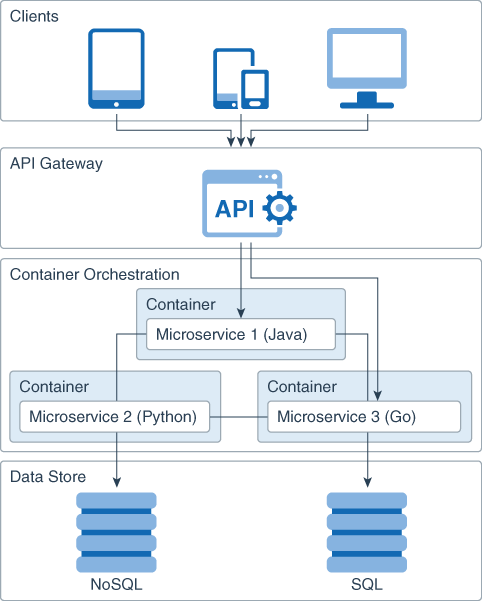
\includegraphics[scale=0.5]{Imagens/microservice_architecture.png}
	\end{center}
	\legend{Fonte: \citeonline{oracle_microservices}}
\end{figure}

Aplicações com uma arquitetura de microsserviços são separadas em partes, chamadas de microsserviços, que são classificadas e se comunicam por meio de uma rede. Microsserviços oferecem capacidades de negócio (funcionalidades relacionadas às regras de negócio da aplicação) ou capacidades de plataforma (funcionalidades relacionadas ao ambiente de execução da aplicação), tratando um aspecto em particular da aplicação. Eles se comunicam por meio de APIs bem definidas, contratos de dados, e configurações. O "micro" em microsserviços faz referência não ao tamanho do serviço, mas sim ao seu escopo de funcionalidade. Eles oferecem apenas uma determinada funcionalidade, tornando-se especialistas nela. Assim sendo, microsserviços não necessariamente devem ser pequenos em tamanho, mas fazem apenas uma tarefa e a fazem eficientemente. 
 
Sendo especialistas em apenas uma tarefa, microsserviços têm características e comportamentos que os diferenciam de outras arquiteturas orientadas a serviços, os quais serão discutidos no \autoref{chapter-caracteristicas}.

A \autoref{figura_arquitetura_microsservicos} exemplifica uma aplicação com arquitetura de microserviços. Inicialmente os usuários da aplicação (camada \emph{Clients}) fazem requisições à api para obter as informações desejadas. O \emph{API Gateway} - que é reponsável por integrar os serviços e será melhor discutido no \autoref{chapter-boas-praticas} - fará as devidas requisições para os devidos microsserviços (localizados na camada \emph{Container Orchestration}). Esses microsserviços então buscarão a informação necessária no devido banco de dados (camada \emph{Data Store}).

% A ilustração mostra as camadas da arquitetura de microsserviços. A primeira camada é a camada do cliente, que contém: os computadores, laptops e dispositivos móveis. A segunda camada é a camada do gateway de API, que redireciona as solicitações do cliente para os microsserviços apropriados. A terceira camada é a camada de orquestração de contêineres, com todos os microsserviços agrupados dentro de uma orquestração de contêineres. Cada um dos microsserviços está em contêiner. Eles se comunicam com os clientes por meio do gateway de API. A quarta camada é a camada de armazenamento de dados. Cada um dos microsserviços em contêiner que implementam persistência se comunica a apenas um armazenamento de dados. Os armazenamentos de dados exibidos são NoSQL e SQL.


% Microsserviços são uma abordagem arquitetônica e organizacional do desenvolvimento de software na qual o software consiste em pequenos serviços independentes que se comunicam usando APIs bem definidas. Esses serviços pertecem a pequenas equipes autossuficientes.

% A arquitetura de microsserviços (AMS) está ganhando força no desenvolvimento e entrega de aplicações de software como um conjunto de pequenos serviços granulares que podem ser integrados por meio de mecanismos de comunicação leve, normalmente APIs RESTful [10]. Microsserviços são componentes pequenos e facilmente entendíveis que possuem capacidades de negócio no meio dos serviços [11]. Esses serviços podem ser escalados independentemente (já que são desacoplados) pela implementação de \texttt{stacks} de tecnologias diferentes [2]. Muitos pesquisadores e praticantes dizem que AMS é uma evolução da Arquitetura orientada a serviços (AOS), como visto no contexto de serviços independentes/auto-suficientes e de natureza leve [12]. Por outro lado, AMS pode ser diferenciada da AOS em termos de compartilhamento de componentes, comunicação de serviços, mediação de serviços, e acesso remoto aos serviços [13]. (Bar, f., 2018, tradução nossa). \cite{WASEEM2020110798}
% % AOS é construida com base na ideia de compartilhar o máximo possível, enquanto AMS, o mínimo possível [13, 14]. AMS usa um estilo coreografico para comunicação inter-serviços, enquanto AOS aplica um estilo de orquestração para coordenação de serviços. Para mediação de serviços, AMS usa a camada de API que atua como uma fachada para o serviço, enquanto AOS adota o conceito de um \texttt{middleware} mensageiro para coodenação de serviços. Além disso, AMS em grande parte depende do protocolo REST e mensageria simples como protocolo de acesso remoto ao serviço; entretanto, AOS consegue lidar com diferentes tipos de protocolo de acesso remoto, incluindo mensageria simples para acessar serviços remotos [13].

\section{Trabalhos relacionados}

\subsection{{Microservices, IoT and Azure, por Bob Familiar - capítulo 2: What is a microservice}}

O capítulo 2 do livro de Bob Familiar descreve o que é um microsserviço, suas características e implicações, benefícios, e desafios. 

"Microservices do one thing and they do it well". Como é explicado por \citeonline{Familiar2015} , microsserviços representam business capabilities definidos usando o design orientado a domínio, são testados a cada passo do \emph{pipeline} de implantação, e lançados por meio de automação, como serviços independentes, isolados, altamente escaláveis e resilientes em uma infraestrutura em núvem distribuída. Pertecem a um time único de desenvolvedores, que trata o desenvolvimento do microsserviço como um produto, entregando software de alta qualidade em um processo rápido e iterativo com envolvimento do cliente e satisfação como métrica de sucesso.

\subsection{A Systematic Mapping Study on Microservices Architecture in DevOps, por Waseem, M., Liang, P. e Shahin, M.}

Esse trabalho tem o objetivo de sistematicamente identificar, analisar, e classificar a literatura sobre microsserviços em DevOps.

Inicialmente o leitor é contextualizado no mundo dos microsserviços e a cultura DevOps. Os autores usam a metodologia de pesquisa de um estudo de mapeamento sistemático da literatura publicada entre Janeiro de 2009 e Julho de 2018. Após selecionados 47 estudos, é feita a classificação deles de acordo com os critérios definidos pelos autores, e então é feita a discussão sobre os resultados obtidos - são expostos a quantidade de estudos sobre determinados tópicos em microsserviços, problemas e soluções, desafios, métodos de descrição, design patterns, benefícios, suporte a ferramentas, domínios, e implicações para pesquisadores e praticantes.

Os principais resultados são: (1) São identificados Três temas de pesquisa em AMS com DevOps “desenvolvimento e operações de microsserviços em DevOps”, “abordagens e suporte a ferramentas para sistemas baseados em AMS em DevOps”, e “Experiência de migração de AMS em DevOps”. (2) São identificados 24 problemas e apontadas suas respectivas soluções com respeito a implementação de microsserviços com DevOps. (3) A AMS é descrita princiapalmente usando caixas e linhas. (4) A maioria das qualidades da AMS são afetadas positivamente quando aplicadas com DevOps. (5) 50 ferramentas que suportam a construção de sistemas baseados em AMS são apontados. (6) A combinação da AMS e DevOps tem sido aplicada em uma ampla variedade de domínios de aplicações.


(Comparar cada trabalho com o meu trabalho. Coisas que eles não abordam e que eu abordo)

\chapter{Características}\label{chapter-caracteristicas}

\chapterprecis{Este capítulo aprensenta as propriedades e as vantagens dos microsserviços, assim como os desafios que acompanham suas implementações.}\index{sinopse de capítulo}

\section{Propriedades dos microsserviços}

\subsection{Autonomia e Isolamento}
Autonomia e isolamento significa que microsserviços são unidades auto-contidas de funcionalidade com dependências de outros serviços fracamente acopladas e são projetados, desenvolvidos, testados e lançados independentemente. O termo autônomo pode ser definido como - existe ou é capaz de existir independetemente das outras partes. O termo isolado, como - separado das outras partes. \cite{Familiar2015}

\subsection{Elasticidade, resiliência, e responsividade}

Microsserviços são reusados entre muitas soluções diferentes e portanto devem ser escaláveis de acordo com o uso. Devem ser resilientes, isso é, ser tolerantes a falhas e ter um tempo de recuperação razoável quando algo der errado. Além disso, devem ser responsivos, tendo um desempenho razoável de acordo com o uso. O termo elástico pode ser definido como - capaz de retornar ao tamanho/formato original depois de ser esticado, comprimido ou expandido. O termo resiliente, como - resistente às mudanças negativas. O termo responsivo, como - Rápido em responder e reagir. \cite{Familiar2015}

\subsection{Orientação-a-mensagens e programabilidade}

Microsserviços dependem de APIs e contratos de dados para definir como interagir com o serviço. A API define um conjunto de endpoints acessíveis por rede, e o contrato de dados define a estrutura da mensagem que é enviada ou retornada. O termo orientado-a-mensagens pode ser definido como - Software que conecta sistemas separados em uma rede, carregando e distribuindo mensagens entre eles. O termo programável, como - Obedece a um plano de tarefas que são executadas para alcançar um objetivo específico. \cite{Familiar2015}

\subsection{Configurabilidade}

Microsserviços devem provêr mais do que apenas uma API e um contrato de dados. Para que seja reusável e para que possa resolver as necessidades do sistema que o use, cada microsserviço tem níveis diferentes de configuração, e esta configuração pode ser feita de diferentes formas. O termo configurável pode ser definido como - Projetado ou adaptado para formar uma configuração ou para algum propósito. \cite{Familiar2015}

\subsection {Automação}

O ciclo de vida de um microsserviço deve ser totalmente automatizado, desde o planejamento (projeto) até a implantação. O termo automatizado pode ser definido como - Funcionar sem precisar ser controlado diretamente. \cite{Familiar2015}

\section{Vantagens}

\subsection{Evolução}

Quanto maior e mais antigo o software, mais difícil é de dar manutenção, e monólitos envelhecem com maior velocidade do que microsserviços. Entretanto, é possível migrar de um sistema monolítico para a arquitetura de microsserviços aos poucos, um serviço por vez, identificando capacidades de negócio, implementando-as como um microsserviço, e integrando com uso de padrões de baixo acoplamento. Ao longo do tempo, mais e mais funcionalidades podem ser separadas e implementadas como microsserviço, até que o núcleo da aplicação monolítica se transforme em apenas um outro serviço, ou um microsserviço. \cite{Familiar2015}

\subsection{Possibilidade de uso de diferentes ferramentas}

Cada microsserviço disponibiliza suas funcionalidades por meio de APIs e contratos de dados em uma rede. A comunicação independe da arquitetura que o microsserviço faz uso, então cada microsserviço pode escolher seu sistema operacional, linguagem e banco de dados. Isso é especialmente valioso para times com dificuldade de comunicação, pois cada time precisa apenas de conhecimento da arquitetura do microsserviço em que trabalha. \cite{Familiar2015}

\subsection{Alta velocidade}

Com um time responsável por cuidar do ciclo de desenvolvimento e sua automação, a velocidade com que microsserviços podem ser desenvolvidos é muito maior do que fazer o equivalente para uma solução monolítica. \cite{Familiar2015}

\subsection{Reusável e combinável}

Microsserviços são reusáveis por natureza. Eles são entidades independentes que provêm funcionalidades em um determinado escopo por meio de padrões de internet aberta. Para criar soluções para o usuário final, multiplos microsserviços podem ser combinados. \cite{Familiar2015}

\subsection{Flexibilidade no ambiente de execução}

A implantação de microsserviços é altamente dependente de sua automação. Para garantir flexibilidade de ambiente de execução, essa automação pode incluir configuração de cenários diferentes de uso, não apenas para produção, mas também para desenvolvimento e testagem, possibilitando que o microsserviço tenha o melhor desempenho em diversos cenários. Para tanto, é necessário o uso de ferramentas que configurem essa flexibilidade. \cite{Familiar2015}. Tais ferramentas serão melhor discutidas no \autoref{chapter-ferramentas}.

\subsection{Flexibilidade na escolha de tecnologias}

Cada microsserviço pode ser desenvolvido usando uma linguagem de programação e estrutura que melhor se adapte ao problema que ele é projetado para resolver, o que oferece mais possibilidades de tecnologias para usar. \cite{oracle_microservices}

\subsection{Versionável e substituível}

Com o controle completo dos cenários de implantação, é possível manter versões diferentes de um mesmo serviço rodando ao mesmo tempo, proporcionando retrocompatibilidade e fácil migração. Além disso, serviços podem ser atualizados ou mesmo substituidos sem ocasionar indisponibilidade do serviço. \cite{Familiar2015}


\section{Desafios}

De acordo com \citeonline{CAOPLE}, os três grandes desafios do desenvolvimento de aplicações com arquitetura de microsserviços são

1 - Como programar sistemas que consistem de um grande número de serviços executando em paralelo e distribuidos em um conjunto de máquinas;
% how to program systems that consists of a large number of services running in parallel and distributed over a cluster of computers;

2 - Como reduzir a sobrecarga de comunicação causada pela execução de grandes números de pequenos serviços;
%how to reduce the communication overhead caused by executing a large number of small services;

3 - Como sustentar a implantação flexível de serviços em uma rede para conseguir realizar o balanceamento de carga.
%how to support the flexible deployment of services to a network to achieve system load balance.

Esses e outros desafios podem ser dividos em tópicos mais específicos, abordados a seguir.

\subsection{Complexidade}
O uso da arquitetura de microsserviços implica num grande aumento de complexidade não apenas na infraestrutura, mas também em algumas etapas do ciclo de desenvolvimento do software, como no \emph{debug} ou nos testes por exemplo. Consequentemente, muitos outros desafios surgem a partir dessa complexidade. Além disso, o uso de diversas tecnologias pode trazer problemas por inexperiência dos desenvolvedores. De acordo com \citeonline{design-monitoring-testing-waseem}, mais pesquisas são necessárias para lidar com a complexidade dos microsserviços no nível de \emph{design} (projeto), de monitoramento, e de testes, desafios para qual não há soluções dedicadas.

% citar curso alura


% Desvantagens dos microserviços:
% - Maior complexidade de desenvolvimento e infraestrutura;
% - Debug mais complexo;
% - Comunicação entre os serviços deve ser bem pensada;
% - Diversas tecnologias pode trazer problemas por inexperiência dos devs;
% - Monitoramento é crucial e mais complexo;
% - (Criar um microserviço pode ser complexo, e ter demais pode trazer problemas.).

\subsection{Comunicação}

- Comunicação entre os serviços deve ser bem pensada

cross-platform compatibility issues and inconsistent call standards issues in the process of development and call microservices. \cite{ZUO2020102878}

\subsection{[re]Organizaçao}

Organizar o sistema e o time para sustentar uma arquitetura de microsserviços é um grande desafio. Como explica \citeonline{Familiar2015}: 
\begin{citacao}
    If you are part of a command-and-control organization using a waterfall software project management approach, you will struggle because you are not oriented to high-velocity product development. If you lack a DevOps culture and there is no collaboration between development and operations to automate the deployment pipeline, you will struggle. \cite{Familiar2015}
\end{citacao}

\subsection{Plataforma}
Criar o ambiente de execução para microsserviços requer um grande investimento em infraestrutura dinâmica em \emph{data centers} dispersos para garantir maior disponibilidade. Se sua atual plataforma \emph{on-premises} não suporta automação, infraestrutura dinâmica, escalamento elástico e alta disponibilidade, deve-se considerar uma plataforma na núvem. \cite{Familiar2015}. Mais sobre soluções na núvem será discutido no \autoref{chapter-ferramentas}.

\subsection{Identificação com DDD}

Domain-driven design (projeto orientado a domínio) é uma técnica bem consolidada e muito usada no desenvolvimento de software. Entretanto, para aplica-la em microsserviços, é necessário analisar onde cada peça desse padrão de projeto deve ficar. Veja a \autoref{praticas-identificacao-com-ddd} para um possível caminho a ser seguido.

% esse parágrafo não encaixa nas caracteristicas - desafios ?...

\subsection{Testes}

Assim como em qualquer aplicação, o teste é uma parte crucial do seu desenvolvimento. Escrever e testar código não muda muito entre as arquiteturas monolítica e de microsserviços, contudo, nos microserviços existem mais testes a serem executados. Não deve-se testar o microsserviço apenas antes de seu lançamento, mas sim em cada passo do \emph{pipeline} de implantação, sempre automatizando o máximo de etapas possível, para assim garantir uma entrega rápida de software de qualidade. \cite{Familiar2015}

% \subsection{Monitoramento}

\subsection{Descoberta}

Encontrar microsserviços em um ambiente distribuido pode ser feito de algumas maneiras diferentes. A informação pode ser armazenada diretamente no código, pode ser guardada e acessada em um arquivo, ou pode ser construido um microsserviço para encontrar outros microsserviços e disponibilizar suas localizações. Contudo, para prover detectabilidade como um serviço será necessário adquirir um produto de terceiros, integrar um projeto aberto, ou desenvolver sua própria solução. \cite{Familiar2015}

\chapter{Práticas}\label{chapter-boas-praticas}

\chapterprecis{Este capítulo apresenta e discute práticas comumente seguidas no desenvolvimento de aplicações com arquitetura de microsserviços.}\index{sinopse de capítulo}

\section{Começar pela arquitetura monolítica}

% But as with any architectural decision there are trade-offs. In particular with microservices there are serious consequences for operations, who now have to handle an ecosystem of small services rather than a single, well-defined monolith. Consequently if you don't have certain baseline competencies, you shouldn't consider using the microservice style. \cite{martin-fowler-microservice-prereq}

\citeonline{martin-fowler-monolith-first} defende o uso de arquiteturas monolíticas para desenvolver novas aplicações. Mesmo os defensores dos microsserviços dizem que há custos e riscos no uso desta arquitetura, os quais desaceleram o time de desenvolvimento, assim favorecendo monólitos para aplicações mais simples. Esse fato leva a um argumento forte para a escolha de uma arquitetura monolítica mesmo se for acreditado que haverá benefícios mais tarde com o uso da arquitetura de microsserviços, por duas razões. A primeira é conhecida como \emph{Yagni - You're not gonna need it}, ou "Você não precisará disso", um preceito do método ágil \emph{ExtremeProgramming} que diz que uma capacidade que acredita-se ser necessária no futuro não deve ser implementada agora por quê "você não precisará disso". A segunda razão é que microsserviços só funcionarão bem se os limites forem muito bem estabelecidos, e para tanto, constrói-se um monólito primeiro para que se possa descobrir os limites antes de serem impostos grandes obstáculos neles pela divisão dos microsserviços \cite{martin-fowler-monolith-first}.
% pois qualquer refatoração de funcionalidade inter-serviços é muito mais difícil do que uma funcionalidade em um monólito.
% It's a statement that some capability we presume our software needs in the future should not be built now because "you aren't gonna need it". 

Além disso, \citeonline{martin-fowler-microservice-prereq} também afirma que existem 3 pré-requisitos para se adotar uma arquitetura de microsserviços, e que é mais fácil lidar com as operações de um monólito bem definido do que de um ecossistema de pequenos serviços. Assim sendo, pode-se considerar uma boa prática começar pela arquitetura monolítica até que o sistema já esteja bem definido e estes pré-requisitos sejam atendidos - provisionamento rápido, monitoramento básico, e implantação rápida de aplicação - explicados na \autoref{boas-praticas-provisionamento-rapido}, \autoref{boas-praticas-monitoramento-basico} e \autoref{boas-praticas-implantacao-rapida} respectivamente \cite{martin-fowler-microservice-prereq}.

Já \citeonline{dontStartWithMonolith-tilkov} contesta essa prática e afirma que não se deve começar pela arquitetura monolítica se o objetivo for uma arquitetura de microserviços. Ele afirma que o melhor momento para se pensar em divir um sistema é justamente quando ele está sendo construido, e que é extremamente difícil dividir um sistema \emph{brownfield} (sistema desenvolvido a partir de outro pré-existente). Entretanto, ele reconhece que para dividir um sistema, deve-se conhecer muito bem o domínio, e que o cenário ideal para o desenvolvimento de microsserviços é quando se está desenvolvendo uma segunda versão de um sistema existente. \citeonline{martin-fowler-monolith-first} reconhece esses argumentos como válidos e reforça que existem, sim, benefícios de se começar por uma arquitetura de microsserviços, mas ainda existem poucas histórias de aplicações com arquiteturas de microsserviços e mais estudos de casos são necessários para saber como determinar a melhor escolha inicial de arquitetura \cite{dontStartWithMonolith-tilkov,martin-fowler-monolith-first}.
% I’m firmly convinced that starting with a monolith is usually exactly the wrong thing to do. 

% If you are actually able to build a well-structured monolith, you probably don’t need microservices in the first place. Which is OK! I definitely agree with Martin: You shouldn’t introduce the complexity of additional distribution into your system if you don’t have a very good reason for doing so. 

\citeonline{monolith-or-microservices} afirma que para decidir a abordagem arquitetural inicial de uma aplicação é necessário considerar o contexto do negócio, da própria aplicação, e do time que a irá desenvolver, e que existem condições que configuram a melhor escolha. Ele descreve 3 condições que tornam a adoção de uma arquitetura de microserviços para uma nova aplicação uma boa escolha: (1) há necessidade de entrega de serviços rapida e independentemente; (2) parte da plataforma precisa ser extremamente eficiente; e (3) planeja-se aumentar o time. Ele também descreve 3 condições que tornam a adoção de uma arquitetura monolítica uma boa escolha: (1) o time ainda está em crescimento; (2) o produto sendo construído é não comprovado ou é uma prova de conceito; e (3) o time não tem experiência com microsserviços \cite{monolith-or-microservices}.

Percebe-se então que existem tanto razões para se começar pelos microsserviços como razões para se começar com uma arquitetura mais simples. Porém, não foi observado um consenso sobre quais seriam exatamente as razões para adotar ou não uma arquitetura de microsserviços para uma nova aplicação desde o início de seu desenvolvimento. Há nesse ponto, portanto, espaço para mais discussões e pesquisas.

% razões que configuram uma boa escolha para a arquitetura inicial de uma aplicação
% discordância sobre o que é ou não necessário para sustentar uma arquitetura de microsserviços desde o início da aplicação, e quais seriam as razões para se adotar ou não essa arquitetura desde o ínicio da aplicação

\subsection{Provisionamento rápido}\label{boas-praticas-provisionamento-rapido}

No contexto da computação, provisionamento significa disponibilizar um recurso, como uma máquina virtual por exemplo. Para produzir \emph{software}, é necessário provisionar muitos recursos, tanto para os desenvolvedores quanto para o cliente. Naturalmente, o provisionamento é mais fácil na nuvem. Na AWS por exemplo, para conseguir uma nova máquina, basta inicar uma nova instância e acessá-la - um processo muito rápido quando comparado ao \emph{on-premises}, onde precisaria-se comprar uma nova máquina, esperar chegar, configurá-la e só então ela estará pronta. Para alcançar um provisionamento rápido, é necessária automação \cite{martin-fowler-microservice-prereq}.

\subsection{Monitoramento básico}\label{boas-praticas-monitoramento-basico}

Muitas coisas podem dar errado em qualquer tipo de arquitetura, mas em especial nos microserviços pois cada serviço é fracamente acoplado, estando sujeitos não só a falhas no código, mas também na comunicação, na conexão, ou até falhas físicas. Portanto, o monitoramento é crucial nesse tipo de arquitetura para que problemas, especialmente os mais graves possam ser detectados no menor tempo possível. Ademais, o monitoramento também pode ser usado para detectar problemas de negócio, como uma redução nos pedidos de um site de vendas, por exemplo \cite{martin-fowler-microservice-prereq}.

\subsection{Implantação rápida}\label{boas-praticas-implantacao-rapida}

Na arquitetura de microserviços a implantação é feita separadamente para cada microsserviço. Com muitos serviços para gerenciar, ela pode se tornar uma tarefa árdua, portanto será novamente necessário um grande nível de automação nessa etapa, geralmente envolvendo um \emph{pipeline} de implantação, que deve ser automatizado o máximo possível \cite{martin-fowler-microservice-prereq}.

\section{A metodologia de 12 fatores}

A metodologia de 12 fatores para o desenvolvimento de aplicações é um conjunto de regras e diretrizes para o desenvolvimento de aplicativos nativos da nuvem e \emph{software} como um serviço. De acordo com ela, os microsserviços devem respeitar as seguintes orientações: \cite{12factor, oracle_microservices,12fatores-rita}

% Metodologia para construir saas que:
% Usam formatos declarativos para automatizar a configuração inicial, minimizar tempo e custo para novos desenvolvedores participarem do projeto;

% Tem um contrato claro com o sistema operacional que o suporta, oferecendo portabilidade máxima entre ambientes que o executem;

% São adequados para implantação em modernas plataformas em nuvem, evitando a necessidade por servidores e administração do sistema;

% Minimizam a divergência entre desenvolvimento e produção, permitindo a implantação contínua para máxima agilidade;

% E podem escalar sem significativas mudanças em ferramentas, arquiteturas, ou práticas de desenvolvimento.

% Este documento sintetiza toda nossa experiência e observação em uma variedade de aplicações que operam como software-como-serviço. Isto é a triangulação de práticas ideais ao desenvolvimento de software, com uma atenção particular a respeito das dinâmicas de crescimento orgânico de uma aplicação ao longo do tempo, a dinâmica de colaboração entre desenvolvedores trabalhando em uma base de código, e evitando os custos de erosão de software

% A metodologia doze-fatores pode ser aplicada a aplicações escritas em qualquer linguagem de programação, e que utilizem qualquer combinação de serviços de suportes (banco de dados, filas, cache de memória, etc).

% 12-Factor Application - É uma metodologia de desenvolvimento que diz que os logs devem ser um stream de dados. Esses logs podem ser impressos na saída padrão, e um serviço específico de logs coleta esses logs, faz o parse, categorização, relatório e todo processamento necessário - https://12factor.net/

I. Base de Código - Cada microsserviço deve ter uma base de código única e particular, com rastreamento utilizando controle de revisão, e devem ser criadas várias versões implantáveis;

II. Dependências - Cada microsserviço deve declarar e isolar suas dependências;

III. Configurações - Configurações de ambiente devem ser armazenadas fora do microsserviço, para que ele possa decidir a configuração apropriada a ser usada;

IV. Serviços de Apoio - Os microsserviços não devem fazer distinção entre serviços de terceiros e serviços locais;

V. Construir, lançar, e executar - Deve-se separar e distinguir cada etapa do processo de desenvolvimento. Na etapa de construção, o código é transformado em um executável. Na etapa de lançamento, o executável se combina com a configuração atual da implantação, seja teste, desenvolvimento ou produção. Na etapa de execução, o aplicativo é executado no ambiente adequado ao lançamento selecionado;

VI. Processos - Deve-se executar a aplicação como um ou mais processos que não armazenam estado, assim diminuindo o acoplamento e facilitando o escalamento;

VII. Vínculo de porta - Um microsserviço deve ser executado em um container e exposto por meio de portas;

VIII. Concorrência - Cada processo deve ser independente e executado separadamente, para se ter um melhor dimensionamento e possibilidade de executar mais ao mesmo tempo;

IX. Descartabilidade - Deve ser possível iniciar ou interromper a aplicação imediatamente sempre que necessário. Caso a aplicação pare de funcionar, deve ser capaz de iniciar novamente sem perdas;

X. Paridade de desenvolvimento e produção - Deve-se manter os ambientes de desenvolvimento, teste e produção o mais semelhantes possível;

XI. Históricos (\emph{Logs}) - Históricos devem ser tratatos como um fluxo de eventos;

XII. Processos administrativos - Tarefas de administração ou de gerenciamento devem ser executadas como processos únicos.

\section{Produtos, não projetos}

A maioria dos times de desenvolvedores trabalham sob o seguinte modelo de projeto: O objetivo é entregar uma peça de \emph{software}, que quando entregue é considerada como completa. Após isso, o \emph{software} é passado para um time de manutenção e o time que o desenvolveu é desfeito. Os praticantes de microsserviços tendem a evitar esse modelo, em vez disso adotando a ideia de que um time deve ser o dono de um produto - não projeto - durante todo seu ciclo de vida. Um exemplo de empresa que adota esse modelo é a Amazon, exercendo a ideia de "você constroi, você executa", na qual um time de desenvolvimento é totalmente responsável por um \emph{software} em produção (um produto). Dessa forma, o time adquire pleno conhecimento de como seu produto se comporta, e como seus usuários o utilizam, pois também terá que realizar o suporte aos usuários do produto. Essa prática também está ligada a separação da aplicação por capacidades de negócio - em vez de enxergar o \emph{software} como um conjunto de funcionalidades a serem implementadas, cria-se uma relação entre os desenvolvedores e os usuários, na qual a questão é como o \emph{software} pode auxiliar o usuário a aumentar a capacidade de negócio. Tal prática também pode ser aplicada em aplicações monolíticas, embora a divisão em microsserviços facilita a crição de relações entre os desenvolvedores de serviços e seus usuários \cite{martin-fowler-microservices}.

% The product mentality, ties in with the linkage to business capabilities. Rather than looking at the software as a set of functionality to be completed, there is an on-going relationship where the question is how can software assist its users to enhance the business capability.

% There's no reason why this same approach can't be taken with monolithic applications, but the smaller granularity of services can make it easier to create the personal relationships between service developers and their users. \cite{martin-fowler-microservices}

\section{Desenvolver e compartilhar ferramentas}
Em vez de apenas usar um conjunto de padrões definidos para desenvolver microsserviços, é preferível produzir ferramentas úteis que outros desenvolvedores possam usar para resolver problemas similares aos que eles enfrentam. Essas ferramentas geralmente são extraídas de implementações maiores e compartilhadas com um grupo mais amplo, geralmente por meio de um modelo de código aberto. Com o Git\footnote{Git: \url{https://git-scm.com/}} e o GitHub\footnote{GitHub: \url{https://github.com/}} se tornando ferramentas tão populares, práticas de código aberto estão cada vez mais comuns \cite{martin-fowler-microservices}.

A Netflix é um exemplo de organização que segue essa filosofia. Compartilhar código útil e muito bem testado como bibliotecas incentiva outros desenvolvedores a resolver problemas semelhantes de maneiras semelhantes, mas deixa a porta aberta para escolher uma abordagem diferente, se necessário. As bibliotecas compartilhadas tendem a se concentrar em problemas comuns, como armazenamento de dados, comunicação entre processos e automação de infraestrutura \cite{martin-fowler-microservices}.

\section{Descentralização dos dados}

Para o gerenciamento de dados, há a possibilidade de compartilhar um banco de dados entre diferentes microsserviços, mas isso é visto como um anti-padrão. Uma aplicação com arquitetura de microsserviços tem melhor isolamento, segurança e disponibilidade quando cada serviço gerencia seu próprio banco de dados particular, inclusive tendo a possibilidade de ser instâncias diferentes da mesma tecnologia ou usar sistemas de banco de dados totalmente diferentes. Os dados persistidos por esses bancos de dados particulares só devem ser acessados diretamente pelo serviço que o contém, e outros serviços que necessitem desses dados precisarão enviar uma requisição. Com cada serviço tendo seu próprio banco de dados, a escalabilidade do serviço e do seu banco pode ser feita em conjunto. Assim, serviços que recebem poucos acessos podem ter bancos menos potentes e mais baratos, e vice-versa \cite{oracle_microservices,martin-fowler-microservices}.

Entretanto, essa descentralização tem implicações para o gerenciamento de atualizações. Geralmente a abordagem para se garantir consistência nas atualizações é pelo uso de transações quando atualizando múltiplos recursos. Contudo, o uso de transações resultada em um acoplamento temporal, o que é problemático quando se tem muitos serviços. Além disso, transações distribuidas são notoriamente difíceis de implementar, e portanto arquiteturas de microsserviços realizam coordenação sem transações entre serviços, com reconhecimento claro de que consistência pode ser apenas consistência eventual e que problemas serão lidados pela compensação de operações \cite{martin-fowler-microservices}.

% \subsection{Arquitetura orientada por eventos}

% \subsection{CQRS}
% Existe um padrão ...

% - Um padrão de codificação: CQRS - Command Query Resposibility Segregation (Segregação da responsabilidade entre o comando e uma busca)
%     "At its heart, [CQRS] is the notion that you can use a different model to update information than the model you use to read information. For some situations, this separation can be valuable, but beware that **for most systems, CQRS adds risky complexity**."

%     Ou seja, usar um modelo para leitura (busca) e outro modelo diferente para escrita (inserção/edição). É possível ter um banco de dados de escrita e outro de leitura, e fazer uma sincronização entre esses. Essa ideia é muito facilitada usando-se o padrão CQRS.
    
%     . Com leitura e escrita separados, cada parte pode realizar operações mais complexas
%     . O modelo de leitura pode ter informações agregadas de outros domínios
%     . O modelo de escrita pode ter dados sendo automaticamente gerados
%     . Aumenta **muito** a complexidade de um sistema


% Choosing to manage inconsistencies in this way is a new challenge for many development teams, but it is one that often matches business practice. Often businesses handle a degree of inconsistency in order to respond quickly to demand, while having some kind of reversal process to deal with mistakes. The trade-off is worth it as long as the cost of fixing mistakes is less than the cost of lost business under greater consistency. \cite{martin-fowler-microservices}
\section{CI/CD}
CI/CD é um método para entregar aplicações e mudanças nelas aos clientes com frequência. CI é um acrônimo de \emph{Continuous Integration} (integração contínua), e diz respeito à automação de como o novo código feito pelo desenvolvedor chega no repositório principal e se transforma em um artefato lançável. CD é um acrônimo de \emph{Continuous Delivery} e/ou \emph{Continuous Deployment} (entrega contínua e/ou implantação contínua). Entrega contínua diz respeito à automação de como os artefatos se transformam em novas versões lançadas que são implantáveis num ambiente de execução a qualquer hora. Implantação contínua diz respeito a automação de como as novas versões lançadas são de fato implantadas no ambiente de execução. A \autoref{figura-ci-cd} ilustra as definições e limites da integração, entrega e implantação contínua. Apesar de determinar essas definições para o presente trabalho, foram observados conflitos na bibliografia revisada tanto nas definições para os termos CI e CD quanto nos limites do que essas práticas englobam, em particular para o termo CD, que pode significar \emph{Continuous Delivery}, \emph{Continuous Deployment}, ou mesmo os dois. No fim, não é importante se ater à semântica - apenas deve-se lembrar que CI/CD é um processo, muitas vezes visualizado como um \emph{pipeline}, que envolve a adição de um alto nível de automação e monitoramento no desenvolvimento de aplicações \cite{redhat-ci-cd, harness-ci-cd, gitlab-ci-cd}.

CI/CD auxilia profissionais de desenvolvimento e de operações a trabalhar mais eficiente e efetivamente, por diminuir tarefas manuais lentas e processos de aprovação antiquados. Além disso, faz com que os processos sejam previsíveis e repetíveis enquanto diminui o espaço para erro humano. Considerando que o ciclo de vida de um microsserviço deve ser tão automatizado quanto possível, CI/CD é uma prática de extrema importância \cite{gitlab-ci-cd}.

\begin{figure}[htb]
	\caption{\label{figura-ci-cd}CI/CD}
	\begin{center}
	    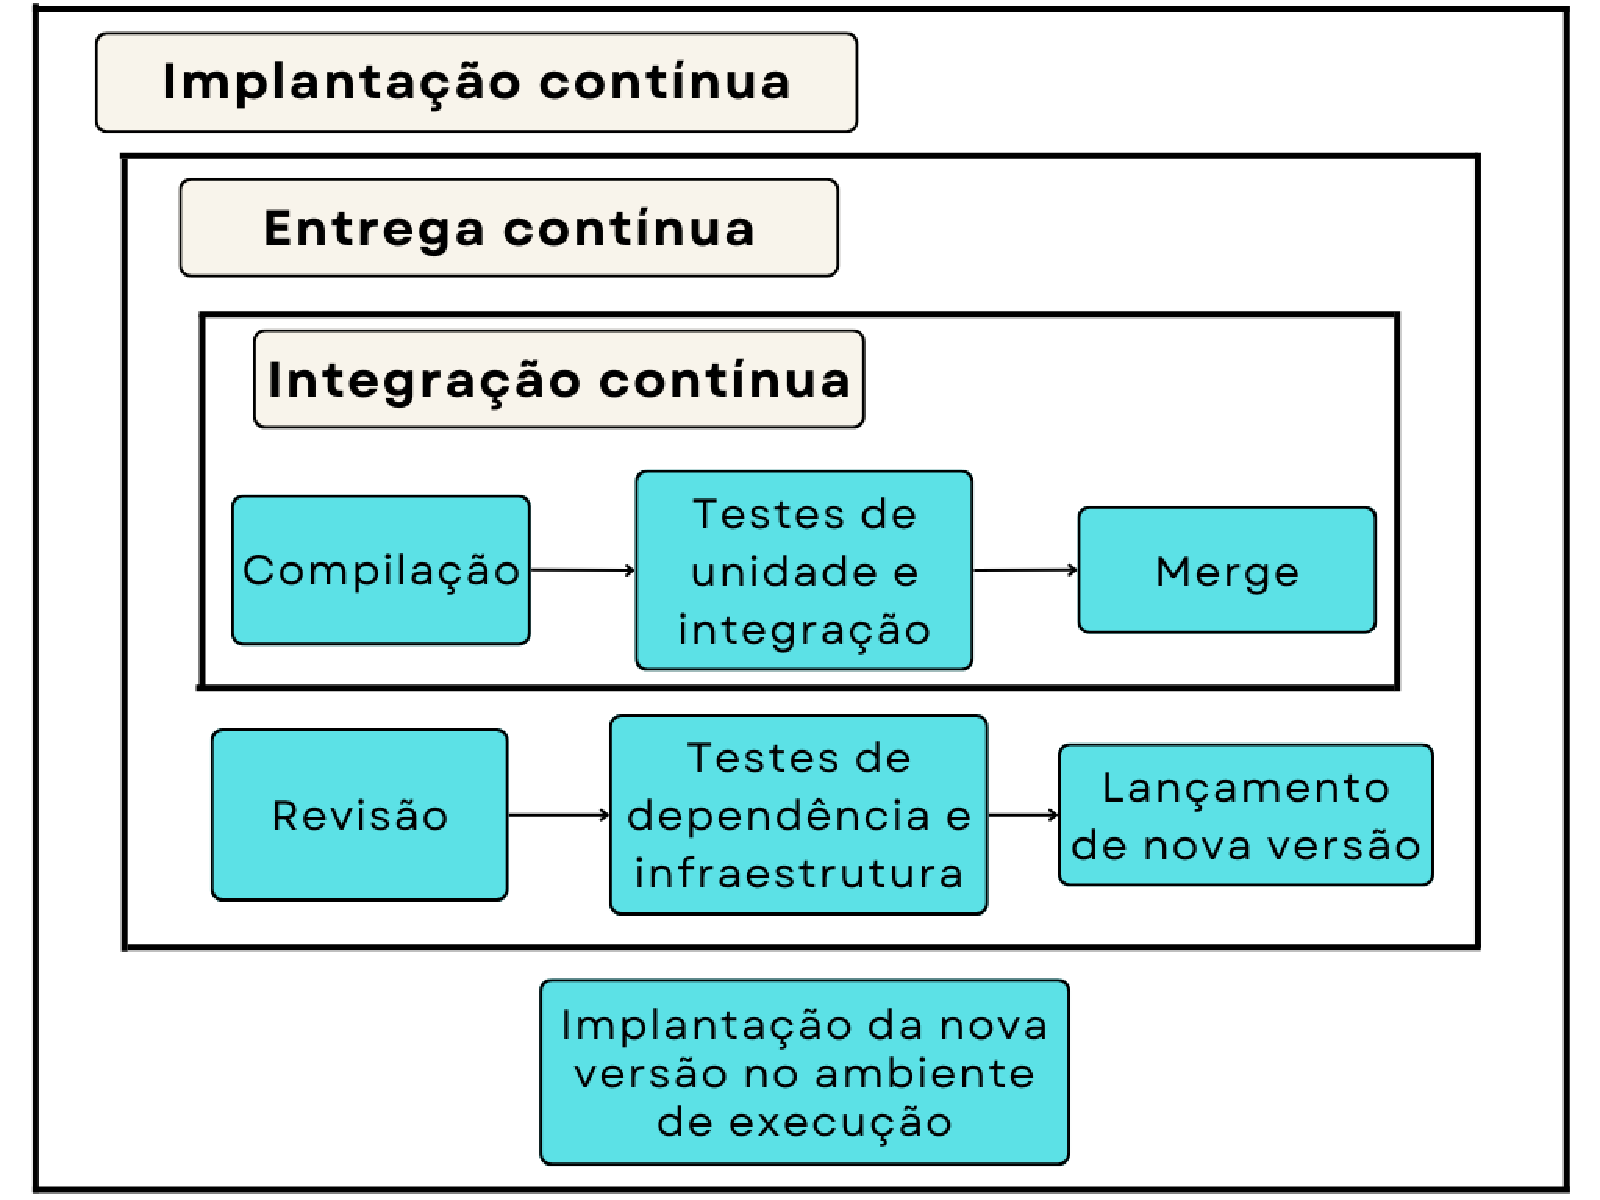
\includegraphics[scale=0.5]{Imagens/ci-cd.pdf}
	\end{center}
	\legend{Fonte: Autor}
\end{figure}
% With continuous delivery, the software is built so that it can be deployed to production at any time. Then you can trigger the deployments manually or move to continuous deployment where deployments are automated as well. \cite{gitlab-ci-cd}

% Continuous Delivery means you ensure every change can be deployed to production. Continuous Deployment means you deploy every change. - Martin fowler https://twitter.com/martinfowler/status/598918601190580224?lang=en

% CI/CD, continuous integration/continuous delivery, é um método para entregar aplicações com frequência aos clientes. Para isso, é aplicada a automação nas etapas do desenvolvimento de aplicações. Os principais conceitos atribuídos a esse método são a integração, entrega e implantação contínuas. Com o CI/CD, é possível solucionar os problemas que a integração de novos códigos pode causar para as equipes de operações e desenvolvimento (o famoso "inferno de integração"). Especificamente, o CI/CD aplica monitoramento e automação contínuos em todo o ciclo de vida das aplicações, incluindo as etapas de teste e integração, além da entrega e implantação. Juntas, essas práticas relacionadas são muitas vezes chamadas de "pipeline de CI/CD" e são compatíveis com o trabalho conjunto das equipes de operações e desenvolvimento com métodos ágeis. citar \url{https://www.redhat.com/pt-br/topics/devops/what-is-ci-cd}

% CI/CD falls under DevOps (the joining of development and operations) and combines the practices of continuous integration and continuous delivery. CI/CD automates much or all of the manual human intervention traditionally needed to get new code from a commit into production such as build, test, and deploy, as well as infrastructure provisioning. With a CI/CD pipeline, developers can make changes to code that are then automatically tested and pushed out for delivery and deployment. Get CI/CD right and downtime is minimized and code releases happen faster. citar \url{https://about.gitlab.com/topics/ci-cd/}

% As you traverse environments from non-prod to the staging environment and eventually to production, the number of endpoints you deploy to increases. Continuous Deployment focuses on the path of least resistance to get the software into the needed environment(s). citar \url{https://harness.io/blog/continuous-delivery-vs-continuous-deployment}

% Being strategic in where to apply parts of your test suite is needed in order to avoid overburdening the Continuous Integration process. A line in the sand should be that Continuous Integration tackles artifact-centric confidence-building (for example, unit tests and artifact scans). Tests that take into account other artifacts and dependencies and/or application infrastructure are better-suited for the Continuous Delivery process. After the build is checked into a central repository, the next step to getting your idea into production is the promotion/deployment process. citar \url{https://harness.io/blog/continuous-delivery-vs-continuous-deployment}

\subsection{CI}
CI (\emph{Continuous Integration} - Integração contínua) é uma prática no desenvolvimento de \emph{software} onde os desenvolvedores integram o código em um repositório compartilhado múltiplas vezes no dia. Muitos times afirmam que essa prática leva a uma grande redução nos problemas de integração e os permite desenvolver \emph{software} coeso mais rapidamente. Além disso, melhora a identificação do progresso do desenvolvimento, facilita a identificação e remoção de falhas e \emph{bugs}, e aumenta a experiência e a confiança do time nos testes e compilação do código desenvolvido. A integração contínua por sí só requer apenas uma ferramenta de controle de versão (como Git\footnote{Git: \url{https://git-scm.com/}}) para ser feita, mas existem práticas bem consolidadas na indústria do desenvolvimento de \emph{software} que auxiliam e incrementam esse processo \cite{martin-fowler-continuous-integration}.

\subsubsection{Manter apenas um repositório fonte}
Deve-se ter um repositório, compartilhado por toda a equipe desenvolvedora, que contém tudo aquilo que é necessário para a construção do projeto, para que seja possível se ter um novo ambiente de desenvolvimento funcional rapidamente. Isso inclui mas não é limitado a - código, \emph{scripts}, migrações e esquemas de bancos de dados, arquivos de propriedades e configurações de IDE. Além disso, o conteúdo do repositório deve estar disponível para todos, assim aumentando a visibilidade e facilitando o monitoramento do progresso do conteúdo \cite{gitlab-ci-cd,martin-fowler-continuous-integration}.

\subsubsection{Automatizar testes de novas compilações}
As integrações de cada novo \emph{commit} no repositório precisam ser compiladas e testadas, o que é uma tarefa árdua e demorada se feita manualmente. Desse modo, deve-se elaborar uma bateria de testes, e executá-la de forma automática a cada nova compilação, para assim detectar falhas rapidamente e aumentar a qualidade do código \cite{gitlab-ci-cd,martin-fowler-continuous-integration}.

\subsubsection{Otimizar a compilação}
Compilações lentas afetam negativamente a integração contínua, atrasando integrações e diminuindo a frequência do \emph{feedback}. Além disso, todas as etapas da compilação devem ser simples de executar, idealmente por meio de um único comando \cite{martin-fowler-continuous-integration}.

\subsubsection{Servidor de integração}
Às vezes não é possível realizar todos os testes necessários na máquina local do desenvolvedor, seja por questões de tempo ou pelo projeto ser muito complexo para ser testado integralmente. Nesse caso, será preciso providenciar um local que será capaz de testar todo o projeto continuamente. Tal local é chamado de \emph{CI Daemon} ou servidor de integração. Esse servidor será responsável por compilar o código a cada \emph{commit}, realizar a bateria de testes e disponibilizar informações e relatórios sobre os passos executados, assim mantendo a qualidade do código e possibilitando a compilação contínua \cite{martin-fowler-continuous-integration}.

\subsubsection{Consertar compilações quebradas imediatamente}
O principal ponto de usar a integração contínua é que a equipe sempre estará trabalhando a partir de uma base estável. Se há uma base instável, é tarefa de toda a equipe resolver o problema o mais rápido possível, pois nenhum novo \emph{commit} poderá ser feito em cima daquela base até que esteja estável e confiável novamente. Geralmente o melhor meio de resolver esse problema é reverter os \emph{commits} problemáticos, trazendo o sistema de volta a um ponto funcional. Não deve-se tentar \emph{debugar} no ramo principal do repositório \cite{martin-fowler-continuous-integration}.

% A continuous integration server acts as a monitor to the repository. Every time a commit against the repository finishes the server automatically checks out the sources onto the integration machine, initiates a build, and notifies the committer of the result of the build. The committer isn't done until she gets the notification - usually an email.

% Not everyone prefers to use a CI server. Jim Shore gave a well argued description of why he prefers the manual approach. I agree with him that CI is much more than just installing some software. All the practices here need to be in play to do Continuous Integration effectively. But equally many teams who do CI well find a CI server to be a helpful tool.

\subsection{CD}
CD significa entrega contínua e/ou implantação contínua, conceitos relacionados e às vezes usados alternadamente. Em ambos os casos, trata-se da automação de fases avançadas do \emph{pipeline} de implantação. A entrega contínua é uma evolução da integração contínua e envolve todo o ciclo do projeto, até a criação da nova versão da aplicação, mas a implantação dessa nova versão no ambiente de execução é feita manualmente. A implantação contínua engloba a entrega contínua e adiciona o passo de automatizar a implantação da nova versão no ambiente de execução. A finalidade da entrega contínua é garantir o mínimo de esforço na implantação de novas alterações, enquanto a da implantação contínua é sempre manter o ambiente de execução atualizado com as últimas alterações. A adoção da implantação contínua deve ser pensada, pois para alguns negócios é preferível uma taxa de implantações mais baixa \cite{gitlab-ci-cd,redhat-ci-cd}.

% Embora seja teoricamente possível realizar entrega contínua sem integração contínua, praticamente é inviável, pois entregar alterações que ainda não foram devidamente integradas no repositório não faz sentido do ponto de vista do desenvolvimento de \emph{software} em equipes 

Os benefícios da entrega contínua incluem: risco reduzido na implantação, pois como as mudanças são menores, há menos possibilidades de problemas, e caso haja, o conserto é mais simples; visualização do progresso, que não será simplesmente por trabalho "completo", mas sim por trabalho entregue; e \emph{feedback} do usuário mais rápida e frequentemente \cite{martin-fowler-continuous-delivery}.

% Um deployment pipeline é um fluxo em que o artefato passa e cada etapa incrementa e agrega mais segurança ao se aproximar do ambiente de produção. Deploys de baixo risco são aqueles experimentais, contínuos, atualizações pontuais acompanhadas. Devemos separar a ideia de "deploy" e "publicação".Otimizar para resiliência é prevenir erros. No contexto de integração e entrega contínua temos o deploy contínuo. As equipes de desenvolvimento normalmente possuem divisões, como as pessoas do QA,deploy e operações. As tarefas são delegadas para os subgrupos durante o projeto. Equipes separadas que mal se comunicam dificultam o andamento do trabalho, aumentam a possibilidade de problemas e atrasam os deploys. A entrega contínua também exige uma mudança no comportamento e na cultura da empresa: as pessoas precisam trabalhar integradas.

% Continuous deployment enables organizations to automatically deploy their applications – eliminating the need for human intervention. With continuous deployment, DevOps teams set the criteria for code releases ahead of time and when those criteria are met and validated, the code is deployed into the production environment. Thanks to this type of automation, organizations are able to be more nimble and get new features into the hands of users faster. \cite{gitlab-ci-cd}

% While you can do continuous integration without continuous delivery or deployment, you can’t really do CD without already having CI in place. That’s because it would be extremely difficult to be able to deploy to production at any time if you aren’t practicing CI fundamentals like integrating code to a shared repo, automating testing and builds, and doing it all in small batches on a daily basis. \cite{gitlab-ci-cd}

% Where Continuous Deployment focuses on the actual deployment, Continuous Delivery focuses on the release and release strategy. An elusive goal would be a “push of a button” to get changes into production. That “push of a button” is Continuous Delivery. \cite{harness-ci-cd}

\section{DevOps}

Por um lado, as equipes de desenvolvimento tentam ser o mais eficientes possível, entregando tarefas completas sempre que possível. Por outro lado, a equipe de operações valoriza a estabilidade, considerando cada alteração como uma possível causa de problemas. Assim, tem-se diferenças importantes no foco do trabalho - uma equipe preza pela velocidade em novas funcionalidades e outra pela estabilidade. Com isso em mente, as equipes precisam aprender a trabalhar em conjunto para conseguir alcançar uma entrega contínua e ao mesmo tempo manter um \emph{software} funcional no ambiente de execução.

DevOps é um movimento cultural que visa a integração e otimização do processo de aprendizagem e cooperação entre os integrantes de equipes relacionadas ao desenvolvimento de \emph{software}. Não se trata de um cargo, mas sim uma visão organizacional de trabalho que tem o objetivo de automatizar o ciclo de desenvolvimento do \emph{software} de modo que seja veloz, seguro e integrado, com foco nas necessidades do usuário e \emph{feedback} rápido. Para tanto, precisa-se de ferramentas para facilitar as automações e monitoramento, mas é importante lembrar que DevOps trata-se mais de um movimento cultural do que uma aparelhagem técnica. Práticas de DevOps, como integração e entrega contínua, são essenciais para o sucesso de aplicações com arquitetura de microsserviços pelos benefícios que traz ao time e ao desenvolvimento da aplicação \cite{gitlab-devops}.

% CI/CD is an essential part of DevOps and any modern software development practice. A purpose-built CI/CD platform can maximize development time by improving an organization’s productivity, increasing efficiency, and streamlining workflows through built-in automation, testing, and collaboration. As applications grow larger, the features of CI/CD can help decrease development complexity. Adopting other DevOps practices — like shifting left on security and creating tighter feedback loops — helps break down development silos, scale safely, and get the most out of CI/CD.

\section{Organização de código}
% Monorepo e polirepo são estratégias de organização de código.
% Para a organização de código no sistema de controle de versionamento, há duas abordagens - monorepo ou polirepo. Também tem a abordagem híbrida.

\subsection{Monorepo}
Monorepo é uma estratégia de organização de código onde usa-se apenas um repositório no sistema de controle de versionamento para gerenciar múltiplos projetos. Ela é usada por diversas grandes empresas como Google, Facebook e Microsoft para gerenciar inúmeros projetos que formam um repositório enorme. O benefício mais tangível dessa abordagem é a simplificação do gerenciamento do versionamento dos projetos - como todos ficam em apenas um repositório, é mais fácil entender o histórico de mudanças e acompanhar o estado da aplicação, também facilitando restaurações de estados anteriores (\emph{rollbacks}). Segundo \citeonline{monorepo-polirepo-nicolas}, o uso dessa estratégia de organização de código também causa um impacto cultural nos times envolvidos com os projetos, encorajando código consistente e de alta qualidade e melhorando a cognição e o trabalho em equipe deles. Por outro lado, essa estratégia também pode causar problemas como: pior desempenho da IDE e de ações como a compilação devido ao grande tamanho do repositório; sobrecarga do servidor de integração devido ao maior número de operações no repositório; aumento do acoplamento entre os projetos caso os desenvolvedores não sigam práticas adequadas para manter o acoplamento baixo; e aumento na complexidade da automação de processos relacionados a integração, entrega e implantação contínua \cite{monorepo-polirepo-semaphoreci, monorepo-do-or-do-not, monorepo-polirepo-nicolas}.

% Por que usar monorepo, que aumenta o acoplamento dos projetos, quando uma grande vantagem dos microsserviços é justamente o baixo acoplamento? 

% Simplifica a documentação . Um único \emph{pipeline} de implantação só que bem mais complexo. Testes de integração e de aceitação são mais fáceis de implementar. Usado por empresas grandes empresas como Google, Facebook e Uber.

% Pros
% 1. Since code for all the services lands in the same place, all issues related to multiple repositories — the proliferation of commits, PRs, code review, etc. disappear. Making the same change across multiple files like Kubernetes templates or logging settings becomes as easy as a global find & replace.
% 2. We also planned on developing a single CI/CD pipeline for all the services, to not have to monitor multiple jobs for failures. More on this below.
% 3. Also, the adoption of a monorepo would not compromise our microservice architecture, like decreasing the number of services would. Despite the move to a single repository each service would remain decoupled from others. All in all, the benefits sounded promising.

% many large enterprises benefit from a mono-repository for source code management because of the improved team cognition that results from eroding barriers between teams and from influencing enhanced teamwork quality.
% it has observed that the benefit of monorepo is the cultural impact. It has asserted that a monorepo facilitates cultural change and enables a holistic team cognition that ensures high quality work and improves communication, while preserving necessary autonomy.
% more research is necessary on source control repository structures and their direct impacts on team cognitions. \cite{monorepo-polirepo-nicolas} 
% a monorepo or polyrepo architecture involves a comparison of tradeoffs while still highlighting that monorepos "encourages consistent and high-quality code, and empowers engineers

\subsection{Polirepo}
Polirepo (também conhecido como multirepo) é uma estratégia de organização de código onde usa-se múltiplos repositórios no sistema de controle de versionamento para o gerenciamento de múltiplos projetos. Na arquitetura de microsserviços isso geralmente significa ter um repositório para cada microsserviço e é a estratégia mais comum de organização de código. Suas vantagens em contraste com o monorepo incluem: tamanho razoável do repositório; escopo do repositório bem definido; definição de permissões diferentes para cada projeto; e operações no repositório têm melhor desempenho. Essa abordagem é mais adequada quando não há necessidade de gerenciar cuidadosamente a versão da aplicação como um todo e esse versionamento é transparente para os usuários \cite{monorepo-polirepo-semaphoreci}.

% Usar um pipeline para cada repo implica em uma microimplantação. É mais cabível para aplicações praticando implantação contínua dos microsserviços, onde o gerenciamento da versão não tem grande importância. Requer mais esforço do que o monorepo mas oferece mais autonomia

% \subsection{Híbrido}

% O que é mais natural é utilizar um repositório para cada projeto, de um tamanho razoável com escopo bem definido. Essa forma de organização é chamada Multi-repo. Há possibilidade de definir permissões de acesso por projeto. clone, commit e build do projeto é mais simples e rápido

% No entanto, nos últimos anos, surgiu uma nova forma de organização dos nossos projetos dentro de repositórios. Empresas grandes de tecnologia como Google e Facebook não utilizam o esquema Multi-repo, porque são empresas que trabalham em inúmeros projetos de maneira concomitante. Empresas que atuam com outra dimensão de projetos utilizam o Mono-repo, ou seja, um único e gigantesco repositório que acumula todos os projetos.

% A desvantagem do segundo modelo é o repositório precisará ser realmente grande, e o build pode ser lento, talvez nem o Git seja mais a ferramenta adequada para fazer o controle de versões para esta situação. Contudo, como temos apenas um grande repositório temos uma administração relativamente mais simples, então a verificação de padrões é facilitada. A refatorações são globais, afinal estão todos dentro da mesma base. 

% \subsection{Estratégias de ramificação} <<

\section{Implantação em containers}

Containers configuram isolamentos lógicos em uma máquina. Eles são leves e altamente flexíveis, permitindo serem parados, alterados e reiniciados rapidamente. Depois de construido o microsserviço, recomenda-se lançá-lo dentro de um container para torná-los padronizados, leves, seguros e evitar interferências com outros microsserviços. Uma opção de mecanismo de gerenciamento de containers é o Docker\footnote{Docker: \url{https://www.docker.com/}} \cite{oracle_microservices}.

% A container is a standardized unit of software, used to develop, ship and deploy applications. Containers are managed using a container engine, such as Docker. The container engine provides the tools that are necessary to bundle all the application dependencies as a container. You can use the Docker engine to create, deploy, and run your microservices applications in containers. Microservices running in Docker containers have the following characteristics:

% Standard: The microservices are portable. They can run anywhere.
% Lightweight: Docker shares the operating system (OS) kernel, doesn’t require an OS for each instance, and runs as a lightweight process.
% Secure: Each container runs as an isolated process. So the microservices are secure.

% The process of containerizing a microservice involves creating a Dockerfile, creating and building a container image that includes its dependencies and the environmental configuration, deploying the image to a Docker engine, and uploading the image to a container registry for storage and retrieval. \cite{oracle_microservices}

\section{Testes}

Tradicionalmente uma compilação engloba tudo que é necessário para que um programa possa executar. Entretanto, só porque um programa executa não significa que ele fará o que se esperava. Para isso deve-se testar o programa, idealmente de forma automática e para toda funcionalidade, assim falhas e \emph{bugs} podem ser descobertos antes de serem lançados. Em uma arquitetura de microsserviços, o processo de testes deve englobar várias estratégias diferentes de testes. Essas estratégias podem incluir testes funcionais, como um teste de unidade, ou testes não-funcionais, como um teste de desempenho. Usar múltiplas estratégias de testes aumenta as chances da aplicação operar com sucesso em ambientes e plataformas diferentes. De acordo com \citeonline{design-monitoring-testing-waseem}, testes de unidade e testes fim-a-fim são as estratégias de testes mais usadas no desenvolvimento de microsserviços \cite{martin-fowler-continuous-integration,Familiar2015}.

% Testes fazem parte da construção do software. Devem ser realizados antes do commit. TDD pode ajudar neste processo. Deve-se prezar por um bom desempenho em testes, pois testes demorados podem ser uma barreira para a integração contínua. Testes automatizados são essenciais para a integração contínua.
% We identified 12 testing strategies (see Table 28), which are listed in our survey question, from the literature (e.g., [9, 6, 61, 63, 64, 65, 66, 67]).

Além de usar os métodos mais comuns de testes, deve-se também testar os microsserviços conforme passam pelo \emph{pipeline} de implantação. Isso inclui: \cite{Familiar2015}

- Testes internos: Testar as funções internas do serviço, inclusive uso de acesso de dados, e caching;

- Teste de serviço: Testar a a implementação de serviço da API. Essa é uma implementação privada da API e seus modelos associados;

- Teste de protocolo: Testar o serviço no nível de protocolo, chamando a API sobre o determinado protocolo (geralmente HTTP);

- Teste de composição: Testar o serviço em cooperação com outros serviços no contexto de uma solução;

- Teste de escalabilidade/taxa de transferência: Testar a escalabilidade e elasticidade do microsserviço implantado;

- Teste de tolerância a falha: Testar a capacidade do microsserviço de recupera-se após uma falha;

- Teste de penetração: Trabalhar com uma empresa terceirizada de segurança de \emph{software} para realizar testes de penetração no sistema.

\section{Comunicação}

Na construção de estruturas de comunicação entre diferentes processos, nota-se muitos produtos e abordagens que enfatizam o emprego de grande inteligência no próprio mecanismo de comunicação. Um exemplo disso é o Enterprise Service Bus (ESB), onde os mecanismos dessa abordagem geralmente incluem recursos sofisticados para roteamento, tratamento e transformação de mensagens e aplicação das regras de negócios \cite{martin-fowler-microservices}.

A comunidade de microsserviços favorece uma abordagem alternativa - \emph{endpoints} inteligentes e canais simples. Os aplicativos criados a partir de microsserviços visam ser o mais desacoplados e coesos possível - eles possuem sua própria lógica de domínio e agem mais como filtros - recebendo uma solicitação, aplicando a lógica conforme apropriado e produzindo uma resposta. Isso é feito usando protocolos REST simples em vez de protocolos complexos como \emph{Web Service Choreography} ou orquestração por uma ferramenta central \cite{martin-fowler-microservices}.

Requisições HTTP em conjunto com uma API de recursos é o método mais usado para realizar comunicação síncrona na arquitetura de microsserviços. Uma requisição HTTP é feita por um cliente para um dado \emph{host} em um servidor, com o propósito de acessar um recurso nesse servidor. Por usar o \emph{Transmition Control Protocol} (TCP), é um método de comunicação confiável, mas não tão eficiente quanto poderia ser \cite{martin-fowler-microservices}.

Para comunicação assíncrona, filas de mensagens são amplamente usadas. Quando um serviço precisa enviar informações a outro de modo assíncrono, ele envia uma mensagem para a fila de mensagens, e ela será armazenada até ser processada ou excluída. Cada mensagem é processada uma única vez, por um único consumidor. As filas de mensagens podem ser usadas para dividir um processamento pesado, para armazenar trabalho em \emph{buffers} ou lotes, ou para amenizar picos de cargas de trabalho \cite{amazon-filas-de-mensagens}.

Embora menos comum, chamada de procedimento remoto (RPC) também é utilizado para realizar comunicação síncrona ou assíncrona nos microsserviços. Uma chamada de procedimento remoto se dá quando um programa faz com que um procedimento ou uma sub-rotina execute em um espaço de endereço diferente, comumente em outra máquina numa rede compartilhada. Essa chamada é feita como se fosse um procedimento local, isso é, o programador não precisa explicitar que se trata de um procedimento remoto. gRPC\footnote{gRPC: \url{https://grpc.io/}} é uma ferramenta moderna com alto desempenho que tem ganhado grande popularidade em meio aos praticantes de microsserviços e é considerada um "projeto de incubação" pela Cloud Native Computing Foundation \cite{microsoft-grpc}.

De acordo com \citeonline{design-monitoring-testing-waseem}, \emph{API Gateway} e \emph{Backend for frontend} são os padrões de projeto mais utilizados para lidar com a comunicação de microsserviços. São padrões similares - a diferença é que no \emph{Backend for Frontend} há um \emph{gateway} para cada tipo de cliente. Esses padrões são discutidos na \autoref{boas-praticas-api-gateway}. 

% Considerando que APIs são um tópico essencial na comunicação entre microsserviços, elas serão abordadas em maior profundidade na \autoref{boas-praticas-apis}.

\section{Monitoramento}

Em qualquer aplicação o monitoramento é importante para garantir um bom funcionamento. Entretanto, na arquitetura de microsserviços o monitoramento se torna indispensável e mais complexo. % Automação e monitoramento estão altamente ligados.

% resource usage and load balancing as monitoring metrics, log management and exception tracking as monitoring practices are widely used \cite{design-monitoring-testing-waseem}

\subsection{Históricos}

Um histórico, também conhecido como \emph{logs}, descreve o que aconteceu em determinado sistema e provê informações sobre o estado e a saúde dele. Manter um histórico do microsserviço é uma forma simples e eficiente de se implementar monitoramento, e é fortemente indicado. Para manter históricos, pode-se desenvolver um serviço dedicado a isso, para ser reutilizado onde necessário. Outra possibilidade é utilizar bibliotecas, próprias ou desenvolvidas por terceiros.

Para facilitar a escrita, leitura e operação dos históricos, deve-se padronizar o formato deles em todos os microsserviços e diferenciar entradas de erros, de avisos e de informação. Além disso, eles devem ser agregados e organizados em um único lugar para que possam ser facilmente consultados.

% Pode haver um serviço dedicado para logs, ou um sidecar de logs (pacote instalável).

% Um motivo importante para organizar os logs é rastrear as chamadas de uma execução. Devemos poder reconstruir uma operação a partir de um identificador. Isso é o equivalente à stack-trace de um sistema monolítico.

% Usar ferramentas de gerenciamento (APMs - Application performance management) para visualizar essas stack-traces.

\subsection{Métricas}
Métricas nos permitem saber o que está acontecendo em qualquer momento, e decidir que ações devem ser tomadas a partir disso. Por exemplo, escalar um serviço que recebe muitas requisições ou diminuir um que não. Métricas podem inclusive servir para questões de negócios e de \emph{business inteligence}. 

Enquanto históricos precisam ser desenvolvidos, métricas apenas precisam de instrumentação pois muitas ferramentas já possuem as próprias métricas ou já existem métodos consolidados para as obter. Nos servidores web mais populares, por exemplo, as informações básicas sobre uma requisição já são gravadas por padrão.

É recomendado usar paineis de controle de alto nível para melhorar a visualização e monitoramento do status da aplicação e diversas outras informações operacionais e de negócio a partir de suas métricas \cite{martin-fowler-microservices}.

\section{APIs}\label{boas-praticas-apis}

Considerando que APIs são uma parte crucial no desenvolvimento de microserviços, sendo responsável por grande parte da comunicação que se faz necessária para conectar tantos serviços separados e manter um funcionamento eficiente e livre de falhas, este trabalho explorará diversas práticas no desenvolvimento de APIs.

\subsection{Códigos de status de respostas HTTP}
Esses códigos são números entre 100 e 599, cada um tendo um significado diferente, e cada centena sendo classificada em tipos diferentes de resposta. 100-199 representam respostas de informação. 200-299 representam respostas de sucesso. 300-399 representam tipos de redirecionamentos. 400-499 representam erros por parte do cliente. 500-599 representam erros por parte do servidor. Isso é um padrão definido na seção 10 da RFC 2616 \cite{rfc_http_nielsen_1999}, e facilita com que o cliente entenda o que aconteceu com a requisição à API. Esses códigos devem ser enviados juntos com a resposta à requisição.

\subsection{Troca de dados com JSON}
Atualmente JSON é um dos formatos mais populares para troca de dados na web, pelo fato de ser facilmente lido tanto por humanos quanto por máquinas. Em APIs, JSON é usado para enviar e receber requisições por meio do protocolo HTTP, sendo uma solução robusta para a comunicação entre cliente e servidor. Embora seja derivado do JavaScript, JSON também é suportado por muitas outras linguagens, seja nativamente ou por meio de bibliotecas.  \cite{json_bourhis_2020}

\subsection{Troca de dados com \emph{Buffers} de Protocolo}\label{subsessao-protocol-buffers}
\emph{Buffers} de protocolo, ou \emph{Protocol buffers} é uma ferramenta de código aberto desenvolvida pelo Google que oferece um método de serialização de dados estruturados para envio de informações. Ela é neutra em linguagem e plataforma, é extensível e funciona como alternativa ao JSON na troca de dados. Essa ferramenta serializa os dados a serem enviados de modo a tornar o pacote mais leve e mais rápido, mas introduz uma complexidade extra. Por introduzir essa complexidade na troca de dados e não ser otimizada para quantidades de dados que excedem alguns megabytes, essa ferramenta não é recomendada para todo caso de uso \cite{google-protocol-buffers}.

\subsection{Contratos de dados e versionamento}
Uma API depende de contratos de dados, isso é, uma definição dos dados que serão recebidos e retornados. Esse contrato implica num compromisso de manter o serviço correspondente funcionando e inalterado. Entretanto, é possível desenvolver melhorias ou adicionar funcionalidades sem quebrar o contrato. Para tanto, deve ser feito um versionamento da API e deve ser mantida a transparência com os clientes que a usam. Por exemplo, sempre que algo for alterado é preciso atualizar a documentação.

Para fazer o versionamento, pode-se usar o processo de versionamento de \emph{software} para representar os estados da API. Nesta técnica, usa-se três números para representar a versão, por exemplo "2.3.7". O primeiro representa a versão maior, o segundo, a versão menor, e o terceiro, o patch (pequena atualização para consertar ou melhorar algo) \cite{wiki_software_versioning_2022}.

Em uma API, para cumprir o contrato de dados, apenas modificações aditivas podem ser feitas, tais como novos endpoints ou novos campos opcionais em algum recurso. Quando isso é feito, a versão da API muda de 2.3.7 para 2.4.0 ou para 2.3.8 dependendo do tamanho da mudança. Quando é necessário realizar alterações que descumprem o contrato, deve-se alterar a versão maior da API, por exemplo passando de 2.3.7 para 3.0.0. Nesses casos, é importante manter a versão anterior funcionando e inalterada, criando uma nova rota para acessar a versão nova, para que clientes usando a versão anterior não apresentem falhas.
% citar o curso da alura

\subsection{API Gateway}\label{boas-praticas-api-gateway}
Numa arquitetura de microsserviços, os clientes geralmente consomem funcionalidades de mais de um microsserviço. Se esse consumo é feito do cliente diretamente para o microsserviço, o cliente precisa lidar com várias requisições aos \emph{endpoints}. Quando os microsserviços mudam ou mais microsserviços surgem frequentemente, fica inviável tratar tantos endpoints por parte do cliente. Uma solução para isso é usar um \emph{API Gateway}. 

Um \emph{API Gateway} é um padrão de projeto e funciona como uma porta única de entrada para as APIs de cada microsserviço, padronizando e controlando o acesso aos microsserviços e APIs. Esse gateway fica situado entre o cliente e os microsserviços, e é responsável por redirecionar as requisições recebidas para os microsserviços apropriados, assim o gerenciamento das chamadas pode ser feita em apenas um lugar em vez de em cada API de cada microsserviço. Além disso, nele também podem ser implementadas camadas de segurança e de monitoramento.

Outra vantagem é que esse \emph{API Gateway} pode agregar requisições, permitindo que o cliente envie apenas uma requisição para o \emph{API Gateway} para recuperar informações de diferentes microsserviços, o que normalmente exigiria múltiplas requisições. Nesse caso, quando recebida a requisição do cliente, o \emph{API Gateway} fica responsável por disparar as requisições correspondentes, agregar as respostas e as devolver ao cliente.

Entretando, também há desvantagens no uso desse padrão: (1) cria-se um alto acoplamento entre os microsserviços e o \emph{API Gateway}, (2) surge um possível ponto massivo de falha nesse \emph{API Gateway} e (3) se não escalado adequadamente, esse \emph{API Gateway} pode se tornar um gargalo \cite{microsoft-api-gateway}.

\subsection{Segurança em APIs}

\subsubsection*{Autenticação}

Incluir autenticação em uma API consiste em exigir uma prova de autorização do uso da API. A autenticação nas APIs é indispensável para aumentar a segurança, e existem formas diferentes de implementá-la.

\subsubsection*{Validação de entradas}

Validar entradas significa verificar as requisições que chegam com o intuito de garantir que elas não contém dados impróprios, tais como injeções de SQL ou \emph{scripting} (execução de uma determinada sequência de comandos) entre sites. Essa validação deve ser implementada tanto em nível sintático como em semântico, isso é, tanto impondo correção da sintaxe quanto impondo correção de valores \cite{rapidAPI-twitter}.

\subsubsection*{Certificado Secute Socket Layer (SSL)}
Usar um certificado SSL permite que o protocolo HTTPS seja usado em vez do HTTP, criptografando as informações que estão trafegando, o que adiciona uma camada de segurança \cite{rapidAPI-twitter}.

\subsubsection*{Limitação de taxa de requisições}
Limitar a taxa de requisições é um jeito de proteger a infraestrutura do servidor nos casos de acontecerem grandes fluxos de requisições, tal como em um ataque de \emph{DoS} (negação de serviço). Clientes terão seu acesso bloqueado caso enviem uma quantidade de requisições acima do limite determinado \cite{rapidAPI-twitter}.

\subsubsection*{Compartilhar o mínimo possível}
Compartilhar o mínimo possível é uma medida de segurança genérica que pode ser adotada em qualquer microsserviço. Especificamente nas APIs, deve-se retornar estritamente apenas os dados necessários para o cliente. Muitas ferramentas usadas para implementar APIs incluem por padrão informações como se fossem marcas d'água, mas que podem ser removidas, tal como headers "X-Powered-By", que vazam informações do servidor que podem auxiliar usuários mal-intencionados \cite{rapidAPI-twitter}.

\subsection{Testes isolados}
Testar uma API isoladamente serve para determinar se ela atende a parâmetros pré-definidos ou não. Tais parâmetros podem ser o cumprimento da funcionalidade, a confiabilidade, a latência, o desempenho, e a segurança. Quando um teste de API falha, deverá ser possível saber precisamente onde o problema se encontra, assim aumentando a velocidade de desenvolvimento e a qualidade do produto.

% Why should you perform API testing?
% - Testing your APIs timely helps to ensure your app is up all the time.
% - It helps to detect API security and performance issues.
% Benefits of API Testing
% - When API tests fail, you will know precisely where the issue lies that crashed the system.
% - As data is exchanged via XML or JSON, you can write API tests in your preferred language.
% - API testing also helps to release the next API version faster. \cite{rapidAPI-twitter}

\subsection{Salvar a resposta no \emph{cache}}
Às vezes referido como \emph{cachear}, salvar informações no \emph{cache} melhora o tempo de busca da informação. Em uma API podem haver múltiplas requisições para a mesma informação em um curto intervalo de tempo, e para cada requisição será necessário buscar a informação. Entretanto, se a informação estiver salva no \emph{cache}, não será necessário buscar essa informação, o que melhora o tempo de resposta da API, especialmente em \emph{endpoints} que frequentemente retornam a mesma resposta \cite{rapidAPI-twitter}.

\subsection{Comprimir os dados}
A transferência de cargas grandes pode diminuir a velocidade da API. Comprimir os dados auxilia nesse problema, diminuindo o tamanho da carga e aumentando a velocidade de transferência. Uma possibilidade é usar \emph{buffers} de protocolo (discutido na \autoref{subsessao-protocol-buffers}) \cite{rapidAPI-twitter}.

% There are various compression methods available, a common one being GZIP. \cite{rapidAPI-twitter}

% \subsection{Evitar trazer ou buscar resultados a mais ou a menos}
% Over-fetching results in unnecessary and unusable data, and under-fetching results in an incomplete response. Good architecture, planning, and appropriate API management tools are essential to avoid these. \cite{rapidAPI-twitter}

\subsection{Paginar e filtrar}
A Paginação separa e categoriza resultados, enquanto a filtragem retorna apenas os resultados relevantes de acordo com os parâmetros da requisição. A paginação e filtragem de resultados reduz a complexidade da resposta e facilitam o uso da API \cite{rapidAPI-twitter}.

\subsection{PATCH ou PUT}
Quando é necessário modificar um recurso em uma API, usa-se os métodos HTTP PUT ou PATCH. Enquanto PUT atualiza o recurso inteiro, PATCH atualiza apenas uma parte específica do recurso, assim usando uma carga de dados menor. Portanto, quando possível deve-se usar PATCH em vez de PUT para modificar um recurso \cite{rapidAPI-twitter}.

% \section{Agregando serviços (process agregator pattern)}
% Um padrão popular Agregar serviços de negócio em um único serviço mantém as funções em um nível mais alto. 

% Agrega serviços de negócio (É ainda mais alto nível)

% Fazem as chamadas para os serviços necessários e montam uma resposta adequada

% Deve ter uma lógica de processamento, e não ser apenas um proxy. No mínimo deve unir a resposta de diversos serviços

% Para construir um agregador, define-se um novo modelo para o sistema, que representará os dados agregados como um subnegócio

% A partir deste modelo, pensar na API que fornecerá as operações

% A ideia é relativamente simples, mas a implementação pode ser complexa

% \section{Pontos de entrada para cada tipo de cliente} 
% Gateway específico para determinados clientes

% Foco nas necessidades reais de determinados clientes

% Esses clientes podem ser clientes da API, como clientes HTTP, ou clientes de negócio mesmo

% Por exemplo, em vez de modificar a lógica de negócios, cria-se um novo 'edge', que receberá a resposta e modificará de acordo com a necessidade do cliente

% Uma possibilidade seria trabalhar apenas com edge services, e nenhum API gateway, isso é, não existiria um ponto único de entrada universal, mas sim um para cada tipo de cliente

% Para construir uma edge (ponta), deve-se primeiro Identificar o cliente e suas necessidades, e Construir contratos específicos para o cliente, isso é, ter recursos diferentes para cada cliente. Por exemplo, a URL pode ser diferente de cliente web para clientes mobile.

% \section{Do monólito aos microserviços}

% Separando serviços monolíticos

% - Separando serviços de domínio (Data Service):
%     . Usar Domain-Driven Design (DDD)
%     . Começar modelando o domínio, não pensando na persistância. Definir previamente as regras e o domínio (Programação orientada a interfaces), para então...
%     . Avaliar **quais ações serão disponibilizadas neste serviço**. (Ex: Inserir, editar, recuperar, exibir, etc...)
%     . Construir o serviço, pensando primeiro no contrato
%     . REST e RPC podem andar juntos

% - Separando serviços de negócio (Business Service):
%     . Identificar o processo que deve ser exposto
%     . Identificar os domínios que serão necessários nesse serviço
%     . Defina a API que será utilizada, focando no domínio e não nos dados. (Ex: Passar uma matrícula, e não um ID)
%     . Consumir serviços de domínio para executar os processos

% - Padrões
%     . Strangler pattern
%         ~ Quebrar um monolito, tirando as funcionalidades dele aos poucos
%         ~ Pode-se começar isolando os dados
%         ~ Ou pode-se começar isolando o domínio

%     . Sidecar pattern
%         ~ Compartilhar código sem que seja necessário criar um novo microserviço.
%         ~ Usa-se pacotes a parte, que podem ser facilmente instalados.
%         ~ Esses pacotes só precisam ser alterados em um lugar para ter efeito em todos os microserviços.
%         ~ Ex: pacotes do npm, do composer, do maven, etc

% \subsection{Identificação com DDD}\label{praticas-identificacao-com-ddd}

% a combination of domain-driven design and business capability is the most used strategy to decompose an application into microservices \cite{design-monitoring-testing-waseem}

% Um caminho possível para facilitar a identificação com DDD dos microsserviços seria em vez de projetar os modelos e os contextos limitados (conceito do DDD usado para limitar um domínio, dividindo modelos grandes e explicitando as relações entre eles) separando-os em camadas, deve-se juntar os contextos limitados com seus respectivos modelos, e procurar por possíveis pontos de separação da aplicação - um lugar onde a linguagem muda, por exemplo. Isso resultaria em um ponto de partida para separar as partes e formar uma arquitetura de microsserviços. \cite{Familiar2015}

% If you are currently working with a complex layered architecture and have a reasonable domain model defined, the domain model will provide a roadmap to an evolutionary approach to migrating to a microservice architecture. If a domain model does not exist, you can apply domain-driven design in reverse to identify the bounded contexts, the capabilities within the system. \cite{Familiar2015}

% % Domain-driven design (design orientado a domínio) é uma tecnica bem consolidada e muito usada no desenvolvimento de software. Entretanto, para aplica-la em microsserviços, é necessário analisar onde cada peça desse padrão de projeto deve ficar. Em vez de projetar os modelos e os contextos limitados separando-os em camadas, pode-se juntar os contextos com seus respectivos modelos, e procurar por possíveis pontos de separação da aplicação - um lugar onde a linguagem muda, por exemplo. Isso resultaria em um ponto de partida para separar as partes e formar uma arquitetura de microsserviços. \cite{Familiar2015}

% \subsection{Organização}

% Em uma mudança do monólito para microsserviços, é recomendado que não sejam feitas mudanças grandes e abruptas na sua organização. Em vez disso, deve-se procurar uma oportunidade com uma iniciativa de negócio para testar a fórmula proposta por \citeonline{Familiar2015} : 

% - Formar um pequeno time inderdisciplinar (cross-functional?).

% - Oferecer treinamento e orientação na adoção de práticas ágeis, como o scrum.

% - Oferecer uma localização física separada para esse time trabalhar a fim de não afetá-lo negativamente por politicas internas ou hábitos antigos.

% - Adotar uma abordagem de minimo produto viável para entregar pequenos mas incrementais \emph{releases} de software, usando essa abordagem durante todo o ciclo de vida.

% - Integrar esse serviço com sistemas existentes, usando um acoplamento solto.

% - Percorrer esse ciclo de vida do microsserviço diversas vezes, fazendo as adaptações necessárias até chegar a equipe ficar confortável com o processo.

% - Colocar o time principal em posições de liderança enquanto são formados novos times interdisciplinares para disseminar o conhecimento e a prática.
% \chapter{Ferramentas}\label{chapter-ferramentas}
%https://dzone.com/articles/30top-tools-for-building-microservices-on-all-leve
\chapterprecis{Este capítulo aprensenta ferramentas que podem ser usadas na construção de aplicações com arquitetura de microsserviços}\index{sinopse de capítulo}

% \section{Design, testes, e monitoramento}

% De acordo com \citeonline{design-monitoring-testing-waseem}, mais pesquisas são necessárias para lidar com a complexidade dos microsserviços no nível de \emph{design} (projeto), de monitoramento, e de testes, desafios para qual não há soluções dedicadas.

Ferramentas de código aberto estão seguidas de um asterisco (*).

\section{Linguagens de programação}
Java, JavaScript, Python, Elixir. \footnote{Uma linguagem de programação não pode, por sí só, ser caracterizada como código aberto ou não, mas uma implementação de uma linguagem pode. Para o escopo deste trabalho, todas as implementações mais comuns das linguages de programação citadas são válidas.}

% A programming language isn't in it self open source or not, but an implementation of it might be. Yes, there are open source implementations of Java. Sun's Java implementation (the most popular one), is one of them.

\section{Bancos de dados}

\subsection{Relacionais}
MySQL*, PostgreSQL*, MariaDB*

\subsection{Not-only SQL}
MongoDB*, Couchbase*, Redis*, Amazon DynamoDB

\section{Integração contínua}
% Many software tools are available to support implementing CI/CD practices. These CI/CD tools range from repository management such as Github and Bitbucket, Jenkins for build automation, and Selenium and Katalon Studio for test automation.

% What are some common CI/CD tools?
% CI/CD tools can help a team automate their development, deployment, and testing. Some tools specifically handle the integration (CI) side, some manage development and deployment (CD), while others specialize in continuous testing or related functions.
% One of the best known open source tools for CI/CD is the automation server Jenkins. Jenkins is designed to handle anything from a simple CI server to a complete CD hub.
% Deploying Jenkins on Red Hat OpenShift

% Tekton Pipelines is a CI/CD framework for Kubernetes platforms that provides a standard cloud-native CI/CD experience with containers.
% Deploying Jenkins on Red Hat OpenShift

% Beyond Jenkins and Tekton Pipelines, other open source CI/CD tools you may wish to investigate include:
%     Spinnaker, a CD platform built for multicloud environments.
%     GoCD, a CI/CD server with an emphasis on modeling and visualization.
%     Concourse, "an open-source continuous thing-doer."
%     Screwdriver, a build platform designed for CD.

% Teams may also want to consider managed CI/CD tools, which are available from a variety of vendors. The major public cloud providers all offer CI/CD solutions, along with GitLab, CircleCI, Travis CI, Atlassian Bamboo, and many others.
% Additionally, any tool that’s foundational to DevOps is likely to be part of a CI/CD process. Tools for configuration automation (such as Ansible, Chef, and Puppet), container runtimes (such as Docker, rkt, and cri-o), and container orchestration (Kubernetes) aren’t strictly CI/CD tools, but they’ll show up in many CI/CD workflows. \cite{redhat-ci-cd}

\subsection{Sistema de controle de versão}
Git, VCS

\subsection{Gerenciamento de repositórios}
GitHub, Bitbucket, GitLab

\subsection{Automação de compilação}
Jenkins

\subsection{Testes automáticos}
Selenium

\subsection{Servidor de integração}
CruiseControl*
% Listamos abaixo alguns servidores de integração disponíveis no mercado. Isso não é uma lista ordenada por popularidade e algum outro critério. Alguns servidores são opensource, outros não, alguns são pagos ou podem ser alocados na nuvem e outros só existem para nuvem ou instalação local.

% Em geral, não existe uma bala de prata e a melhor ferramenta é aquela que te serve bem:
%     Jenkins (https://jenkins.io/)
%     GoCD (https://www.gocd.org/)
%     Bamboo (https://www.atlassian.com/br/software/bamboo)
%     Travis CI (https://travis-ci.org/)
%     Team City (https://www.jetbrains.com/teamcity/)
%     Circle CI (https://circleci.com/)
%     Gitlab (https://about.gitlab.com/product/continuous-integration/)
%     AWS Code Pipeline https://aws.amazon.com/codepipeline/
%     Azure (https://azure.microsoft.com/pt-br/services/devops/server/)

% At Thoughtworks, we're big fans of continuous integration servers - indeed we led the original development of CruiseControl and CruiseControl.NET, the widely used open-source CI servers. Since then we've also built the commercial Cruise CI server. We use a CI server on nearly every project we do and have been very happy with the results.

\section{Comunicação}

\subsection{RPC}
gRPC (\url{https://grpc.io/})

\subsection{Mensagens}
RabbitMQ*, Azure Service Bus, Amazon Simple Queue Service, Google Cloud Pub/Sub.

\subsection{Streaming de dados e mensagens}
Apache Kafka*

\subsection{APIs}

\subsubsection{API Gateway}
Tyk*, Amazon API Gateway

\subsubsection{Linguagem de consulta}
GraphQL*

\subsubsection{Documentação}
Swagger Inspector

% \subsection*{GraphQL}
% A query language for your API
% GraphQL is a query language for APIs and a runtime for fulfilling those queries with your existing data. GraphQL provides a complete and understandable description of the data in your API, gives clients the power to ask for exactly what they need and nothing more, makes it easier to evolve APIs over time, and enables powerful developer tools. \cite{GraphQL-site}

\subsubsection{Testes de API}\label{ferramentas-testes-apis}
Postman*, Hoppscotch*, API Fortress

% RapidAPI offers RapidAPI Client for VS Code to test APIs locally inside Visual Studio Code. You can also schedule API tests using RapidAPI Studio.
% programar os testes em uma linguagem de programação
% cURL
% postman
% solução integrada ao VSCode - thunderclient

\section{Provisionamento}

\subsection{de máquinas virtuais}
VirtualBox*

\subsection{de containers}
Docker*

\subsection{na nuvem}
AWS EC2

\subsection{automático}
AWS Launch Templates

% \section{Escalamento}
% AWS Auto Scaling Groups

% \subsection{Ferramentas para segurança em APIs}

% Autenticação - Always use secure authentication methods such as OAuth, JWTs, or API Keys. It's not recommended to use basic HTTP authentication as it sends user credentials with each request. It is considered the least secure method.

% Validação de entradas - Métodos de validação de entrada: JSON and XML Schema validation; Regular expressions;  Data type validators available in framework; Minimum and maximum value range check for numerical inputs;  Minimum and maximum length check for strings.

% \subsubsection{Métodos de autenticação}

% API Keys are unique identifiers assigned to clients, which grant them access to an API. They are passed to the server with every request and authenticate the client. They also provide authorization and can be used to identify a user's individual access permissions. API Keys are long alphanumerical strings designed to be almost impossible to guess. They are passed to servers as a query parameter or in an HTTP request header.

% OAuth is a powerful framework that uses tokens to give apps limited access to a user’s data without needing the user’s password. The tokens used are restricted and only allow access to data that the user specified for the particular app. It works by the user(client) first requesting authorization from the resource owner. The user is then given a unique access token from an authorization server used in each request to the resource server.

% Basic HTTP authentication involves the client passing the user’s username and password with every request. This is done using an HTTP Header. Basic HTTP authentication is generally considered the least secure. However, if you decide to use it, ensure you are using an HTTPS connection. If not, data is a risk of being leaked.

% Ferramenta para rate limiting. \cite{rapidAPI-twitter}

\section{Orquestração}

Docker Swarm*, Kubernetes*, Conductor*, Azure Kubernetes Service (AKS)

% Learn About Orchestrating Microservices Using Kubernetes

% The microservices that are running in containers must be able to interact and integrate to provide the required application functionalities. This integration can be achieved through container orchestration.

% Container orchestration enables you to start, stop, and group containers in clusters. It also enables high availability and scaling. Kubernetes is one of the container orchestration platforms that you can use to manage containers.

% After you containerize your microservices, you can deploy them to Oracle Cloud Infrastructure Container Engine for Kubernetes.

% Before you deploy your containerized microservices application to the cloud, you must deploy and test it in a local Kubernetes engine, as follows:

%     Create your microservices application.
%     Build Docker images, to containerize your microservices.
%     Run your microservices in your local Docker engine.
%     Push your container images to a container registry.
%     Deploy and run your microservices in a local Kubernetes engine, such as Minikube.

% After testing the application in a local Kubernetes engine, deploy it to Oracle Cloud Infrastructure Container Engine for Kubernetes as follows:

%     Create a cluster.
%     Download the kubeconfig file.
%     Install kubectl tool on a local device.
%     Prepare the deployment.yaml file.
%     Deploy the microservice to the cluster.
%     Test the microservice.

% The following diagram shows the process for deploying a containerized microservices application to Oracle Cloud Infrastructure Container Engine for Kubernetes. \cite{oracle_microservices}

\section{Monitoramento}
Logstash*, Middleware, Elastic Stack, Graylog*

\section{Conjunto de ferramentas}
Seneca*, Google Cloud Functions,

\section{Framework arquitetural}
goa*, Kong*

\section{Ferramentas sem servidor}
Claudia, Apache Openwhisk, Serverless, Kubeless, IronFunctions, AWS Lambda, OpenFaaS, Microsoft Azure Functions.

% \section{Plataformas}
% Microsoft Azure is a microservice platform, and it provides a fully automated dynamic infrastructure, SDKs, and runtime containers along with a large portfolio of existing microservices that you can leverage, such as DocumentDb, Redis In-Memory Cache, and Service Bus, to build your own microservices catalog. \cite{Familiar2015}
% AWS
% Uma solução para a sobrecarga na execução de tantos microserviços é a um ambiente de desenvolvimento integrado na linguagem CAOPLE \cite{CAOPLE}. Essa plataforma oferece grande controle sobre a implantação e testagem de microserviços.
\chapter{Plano de Continuidade}

Esta foi a primeira etapa do trabalho. Na próxima etapa, planeja-se: (1) propor uma combinação de ferramentas para o desenvolvimento de aplicações com arquitetura de microsserviços, (2) contextualizar essas ferramentas e apontar os problemas que elas resolvem, (3) desenvolver uma aplicação de exemplo com arquitetura de microsserviços usando as ferramentas propostas e boas práticas discutidas e (4) discutir pontos positivos e negativos das ferramentas usadas nessa aplicação de exemplo. O cronograma de atividades previstas para serem realizadas na disciplina de Trabalho de Conclusão de Curso 2 é apresentado na \autoref{figura-grafico-gantt}.

\begin{figure}[htb]
	\caption{\label{figura-grafico-gantt}Cronograma de atividades que serão desenvolvidas.}
	\begin{center}
	    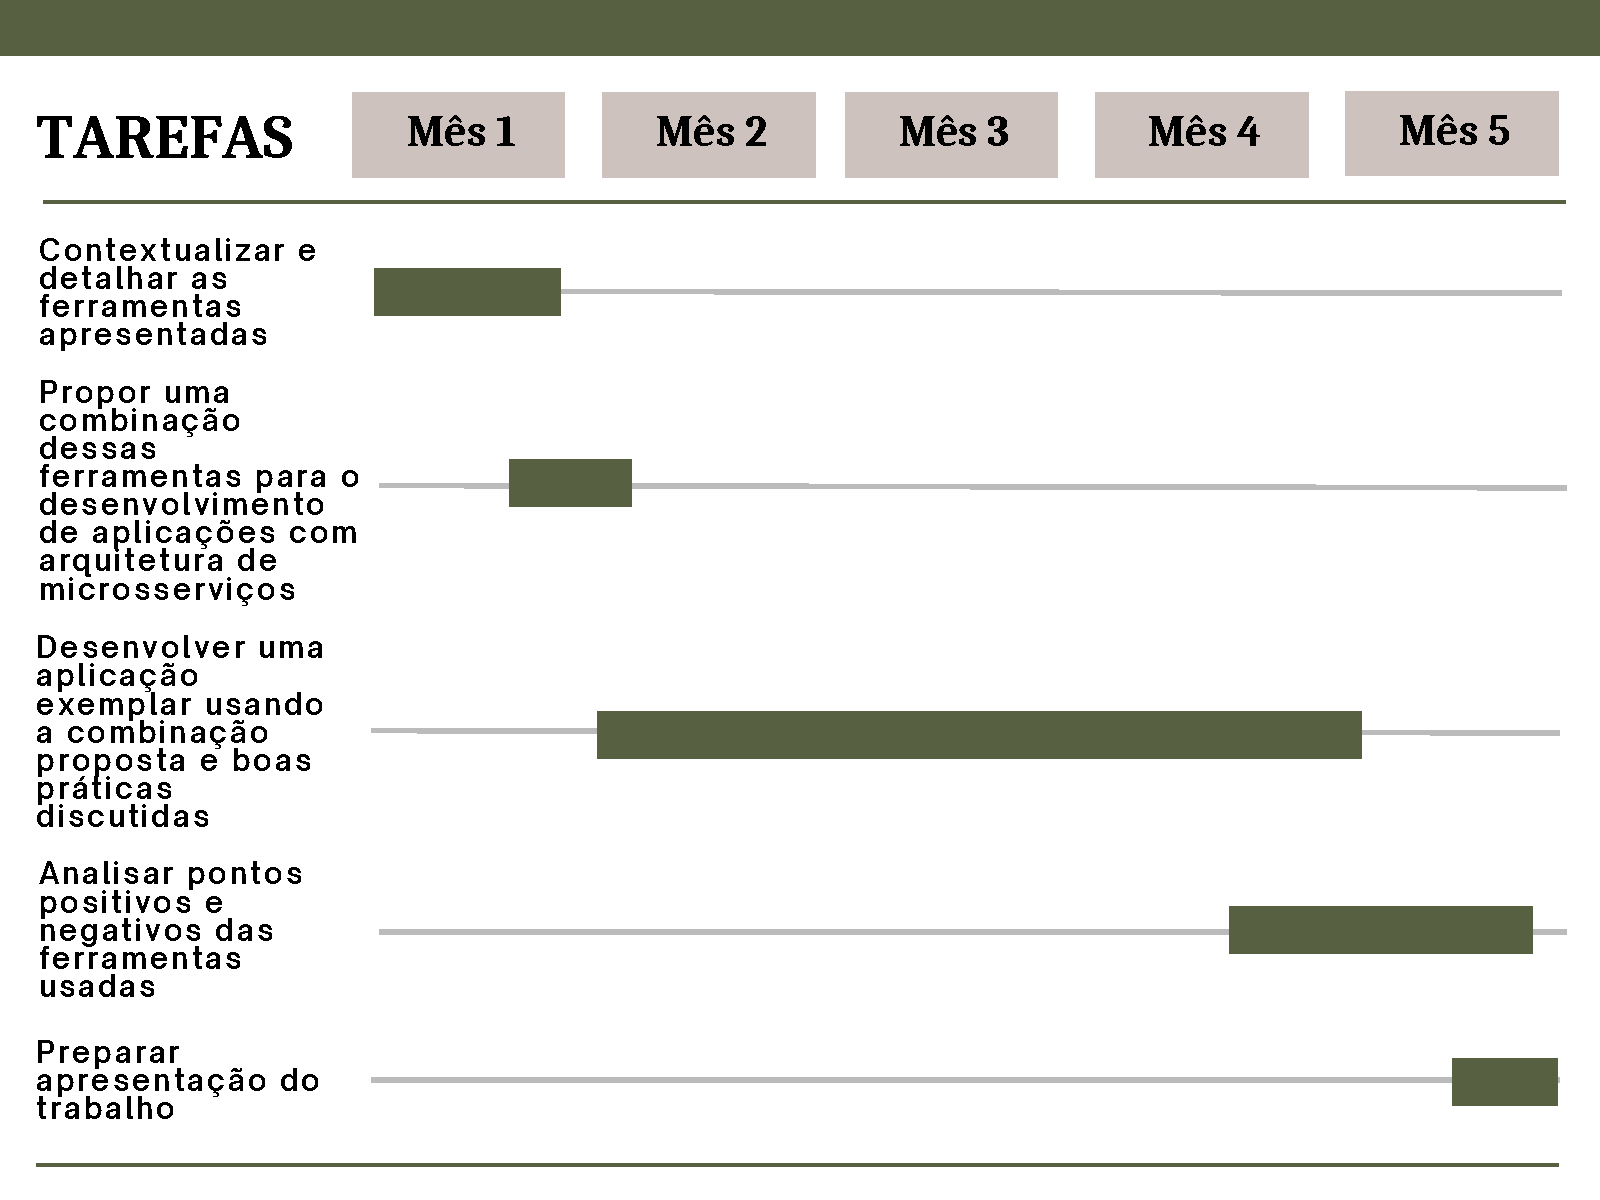
\includegraphics[scale=0.5]{Imagens/grafico-gantt.pdf}
	\end{center}
	\legend{Fonte: Autor}
\end{figure}

\chapter{Conclusão}\label{chapter-conclusao}

Como pôde ser constatado, a escolha da arquitetura de uma aplicação não é uma decisão simples. Assim como quase tudo na computação, trata-se de \emph{tradeoffs}, e para determinar se a arquitetura a ser escolhida é adequada, precisa-se entender e contextualizar seus benefícios, riscos, desvantagens e desafios. Apesar de não existir uma definição formal para a arquitetura de microsserviços, há muitas características que a diferencia de outras abordagens arquiteturais, tais como a componentização, a evolução, e a complexidade.

Foi observada uma ampla concordância entre pesquisadores e praticantes de microsserviços acerca do que é comum, do que é bem-visto, do que é considerado um anti-padrão, e de quais são os desafios no desenvolvimento de aplicações com arquitetura de microsserviços, assuntos os quais foram contextualizados e discutidos neste trabalho. Também foi descoberto um ponto em que há mais espaço para discussão e pesquisa - a prática de se começar uma arquitetura de microsserviços por uma arquitetura monolítica até que a aplicação e seus domínios já estejam bem definidos -, pois foi observado certo nível de discordância entre os autores das bibliográfias revisadas sobre o que é ou não necessário para sustentar uma arquitetura de microsserviços desde o início do desenvolvimento da aplicação, e quais seriam as razões para se adotar ou não essa arquitetura.

A proposta de uma combinação de ferramentas que podem ser usadas no desenvolvimento de aplicações com arquitetura de microsserviços e suas contextualizações ficaram adiadas para serem exploradas na próxima etapa deste trabalho. Também ficaram para a próxima etapa o desenvolvimento de uma aplicação exemplar com arquitetura de microsserviços usando a combinação proposta e a discussão acerca dos pontos positivos e negativos observados no uso dessas ferramentas.

% Foram apresentadas as características mencionadas como imprescindíveis por pesquisadores e praticantes de microsserviços, assim como as que aparecem com mais frequência na literatura. 

% As conclusões constituem a parte final do texto, na qual se apresentam as considerações finais sobre o assunto, se os objetivos foram alcançados, o que se descobriu, quais outras questões surgiram a partir dos resultados e se as hipóteses se confirmaram ou não. Vale lembrar que nenhum trabalho de pesquisa encerra um tema ou problema, por isso, evite fazer afirmações redutoras ou definitivas.

\phantompart
\bibliography{Bibliografia}

%%%%%%%%%%%%%%%%%%%%%%%%%%%%%%%%%%%%%%%%%%%%%%%%%%%%%%%%%%%%%%%%%%%%%%%%%%
% ELEMENTOS PÓS-TEXTUAIS
%%%%%%%%%%%%%%%%%%%%%%%%%%%%%%%%%%%%%%%%%%%%%%%%%%%%%%%%%%%%%%%%%%%%%%%%%%

\postextual

\renewcommand{\chapnumfont}{\chaptitlefont}
\renewcommand{\afterchapternum}{}
%\include{Pos_Textual/Apendices}
%\include{Pos_Textual/Anexos}

\end{document}
